\section{Order statistics}\label{sec:B-orderstats}

Auction data rarely reveal every bidder's value. An ascending auction ends at the price where the
second-to-last bidder drops out, which is the second-highest value. A Dutch auction records only the
winning bid. \emph{Order statistics}, the sorted values of a sample, connect such partial observations to
the distribution of values. The Gumbel distribution of \cref{sec:B-gumbel} arose as the limit of a sample
maximum, and here we study maxima and the other order statistics in finite samples. This section collects their
distribution theory and the identification results built on it. \Cref{ch:auction-theory} uses these tools to derive equilibrium bids and revenues.
\Cref{ch:auction-empirics} uses them to identify and estimate value distributions.

\subsection{Definitions, maxima and minima}\label{sec:B-os-def}

Let $X_1, \dots, X_n$ be i.i.d.\ random variables with continuous CDF $F$, density $f$ and support
$[\underline x, \bar x]$, where the endpoints may be infinite. Sorting the sample from lowest to highest
gives the order statistics
\begin{equation*}
  X_{(1:n)} \leq X_{(2:n)} \leq \dots \leq X_{(n:n)}.
\end{equation*}
Thus $X_{(k:n)}$ is the $k$-th lowest of the $n$ draws, $X_{(n:n)}$ is the maximum and $X_{(1:n)}$ is the
minimum. We write $F_{(k:n)}$ for the CDF of $X_{(k:n)}$ and $f_{(k:n)}$ for its density. The indexing from
lowest to highest follows \citet[Section~2.1]{AtheyHaile2007}. Because $F$ is continuous, two draws coincide
with probability zero, so the inequalities are strict almost surely.

The maximum is at most $x$ if and only if every draw is at most $x$. Independence then gives
\begin{equation}\label{eq:B-os-max}
  F_{(n:n)}(x) = \Pr(X_1 \leq x, \dots, X_n \leq x) = \prod_{m=1}^{n}\Pr(X_m \leq x) = F(x)^n,
\end{equation}
and differentiation gives $f_{(n:n)}(x) = nF(x)^{n-1}f(x)$. The minimum exceeds $x$ if and only if every
draw exceeds $x$, so
\begin{equation}\label{eq:B-os-min}
  1 - F_{(1:n)}(x) = \Pr(X_1 > x, \dots, X_n > x) = \big(1 - F(x)\big)^n.
\end{equation}
Hence $F_{(1:n)}(x) = 1 - (1 - F(x))^n$ and $f_{(1:n)}(x) = n(1 - F(x))^{n-1}f(x)$.

Two special cases recur in auctions. First, bidder $i$ faces $n-1$ rivals, and the highest rival value
$Y_1 = \max_{j \neq i}X_j$ is the maximum of $n-1$ i.i.d.\ draws. By \eqref{eq:B-os-max} its CDF is
$F_{Y_1}(y) = F(y)^{n-1}$. If all bidders use the same strictly increasing bid function, a bidder with value
$v$ therefore wins with probability $F(v)^{n-1}$. Second, the lowest bid wins a procurement auction. Minima
then play the role that maxima play in sales, and the survival function $1 - F$ replaces $F$. For example,
a supplier with cost $c$ undercuts $n-1$ independent rivals with costs drawn from $F_c$ with probability
$(1 - F_c(c))^{n-1}$.

\begin{remark}[Reduction to the uniform case]\label{rem:B-os-quantile}
Let $U_1, \dots, U_n$ be i.i.d.\ uniform on $[0,1]$ and set $X_m = F^{-1}(U_m)$, so that each $X_m$ has CDF $F$
by \cref{lem:B-pit}. The quantile function $F^{-1}$ is nondecreasing, so it preserves the ordering of the
sample. Hence $X_{(k:n)} = F^{-1}(U_{(k:n)})$. In the other direction, $F(X_m)$ is uniform and $F$ is
nondecreasing, so $F(X_{(k:n)})$ has the distribution of $U_{(k:n)}$. Every distributional statement about
order statistics of a continuous parent distribution therefore reduces to a statement about uniform order
statistics.
\end{remark}

\subsection{The \texorpdfstring{$k$}{k}-th order statistic}\label{sec:B-os-k}

For $t \in [0,1]$ and $1 \leq k \leq n$ define
\begin{equation}\label{eq:B-phi}
  \phi_{k:n}(t) = \frac{n!}{(k-1)!\,(n-k)!}\int_0^t u^{k-1}(1-u)^{n-k}\,\dd u.
\end{equation}
This is the CDF of a beta distribution with parameters $k$ and $n-k+1$. \Cref{ch:auction-theory} writes
$\Lambda_n$ for the map $\phi_{n-1:n}$.

\begin{proposition}[Distribution of the $k$-th order statistic]\label{prop:B-os-cdf}
For $k = 1, \dots, n$ and every $x$,
\begin{equation}\label{eq:B-os-cdf}
  F_{(k:n)}(x) = \sum_{m=k}^{n}\binom{n}{m}F(x)^m\big(1 - F(x)\big)^{n-m} = \phi_{k:n}\big(F(x)\big).
\end{equation}
\end{proposition}

\Cref{prop:14-orderstat} proves the formula in two steps. The $k$-th lowest draw is at most $x$ if and only if
at least $k$ of the $n$ draws are. Their number is binomial with parameters $n$ and $F(x)$, which gives the
binomial sum. Its derivative in $F(x)$ telescopes to the integrand of \eqref{eq:B-phi}, and both sides vanish at
$F(x) = 0$. Formula \eqref{eq:B-os-cdf} is equation (5) of \citet{AtheyHaile2002}, who cite
\citet{ArnoldBalakrishnanNagaraja1992}. The chain rule gives the density,
\begin{equation}\label{eq:B-os-density}
  f_{(k:n)}(x) = \phi_{k:n}'\big(F(x)\big)f(x)
  = \frac{n!}{(k-1)!\,(n-k)!}\,F(x)^{k-1}\big(1 - F(x)\big)^{n-k}f(x).
\end{equation}
The density has a multinomial reading. For $X_{(k:n)}$ to fall in $[x, x + \dd x]$, one draw must land in
that interval, $k-1$ draws must fall below $x$ and $n-k$ above. These events have probabilities $f(x)\,\dd
x$, $F(x)^{k-1}$ and $(1 - F(x))^{n-k}$. The multinomial coefficient $\frac{n!}{(k-1)!\,1!\,(n-k)!}$ counts
the ways of assigning the draws to the three groups. The cases $k = n$ and $k = 1$ recover the maximum and
the minimum.

\begin{example}[The second-highest draw]\label{ex:B-second-highest}
Take $k = n-1$. By \cref{rem:B-os-quantile} it suffices to consider uniform draws. The second-highest of $n$
uniform draws is at most $t$ when at least $n-1$ of them are at most $t$. Either all $n$ are, with probability $t^n$, or exactly $n-1$ are, with probability
$nt^{n-1}(1-t)$, where the factor $n$ counts the choices of the single draw above $t$. Hence
\begin{equation*}
  \phi_{n-1:n}(t) = nt^{n-1}(1-t) + t^n.
\end{equation*}
The integral formula \eqref{eq:B-phi} gives the same answer:
\begin{align*}
  \phi_{n-1:n}(t) &= n(n-1)\int_0^t u^{n-2}(1-u)\,\dd u \\
  &= n(n-1)\Big[\frac{t^{n-1}}{n-1} - \frac{t^n}{n}\Big] \\
  &= nt^{n-1} - (n-1)t^n,
\end{align*}
which equals $nt^{n-1}(1-t) + t^n$. Differentiating the last form,
\begin{equation*}
  \phi_{n-1:n}'(t) = n(n-1)t^{n-2} - n(n-1)t^{n-1} = n(n-1)t^{n-2}(1-t) > 0 \qquad \text{for } t \in (0,1).
\end{equation*}
In a second-price or ascending auction with symmetric independent private values, the price is the
second-highest value. Its CDF is therefore $nF(v)^{n-1}(1 - F(v)) + F(v)^n$ (\cref{ch:auction-theory}).
\end{example}

\begin{proposition}[Uniform order statistics]\label{prop:B-os-uniform}
The random variable $U_{(k:n)} = F(X_{(k:n)})$ has the beta distribution with parameters $k$ and $n-k+1$.
Its mean and variance are
\begin{equation}\label{eq:B-os-beta-moments}
  \E\big[U_{(k:n)}\big] = \frac{k}{n+1}, \qquad \Var\big(U_{(k:n)}\big) = \frac{k(n-k+1)}{(n+1)^2(n+2)}.
\end{equation}
\end{proposition}

\begin{proof}
By \cref{rem:B-os-quantile}, $U_{(k:n)}$ is the $k$-th order statistic of $n$ uniform draws. With $F(u) = u$
on $[0,1]$, the density \eqref{eq:B-os-density} becomes $\frac{n!}{(k-1)!\,(n-k)!}u^{k-1}(1-u)^{n-k}$, the
beta density with parameters $k$ and $n-k+1$. For the moments we use the beta integral
$\int_0^1 u^a(1-u)^b\,\dd u = \frac{a!\,b!}{(a+b+1)!}$ for nonnegative integers $a$ and $b$. The mean is
\begin{equation*}
  \E\big[U_{(k:n)}\big] = \frac{n!}{(k-1)!\,(n-k)!}\cdot\frac{k!\,(n-k)!}{(n+1)!} = \frac{k}{n+1}.
\end{equation*}
The second moment is
\begin{equation*}
  \E\big[U_{(k:n)}^2\big] = \frac{n!}{(k-1)!\,(n-k)!}\cdot\frac{(k+1)!\,(n-k)!}{(n+2)!}
  = \frac{k(k+1)}{(n+1)(n+2)}.
\end{equation*}
Subtracting the squared mean,
\begin{equation*}
  \Var\big(U_{(k:n)}\big) = \frac{k(k+1)}{(n+1)(n+2)} - \frac{k^2}{(n+1)^2}
  = \frac{k\big[(k+1)(n+1) - k(n+2)\big]}{(n+1)^2(n+2)} = \frac{k(n-k+1)}{(n+1)^2(n+2)}.
\end{equation*}
\end{proof}

The means say that $n$ uniform draws split $[0,1]$ into $n+1$ spacings of equal expected length
$\frac{1}{n+1}$. The variances say that extremes are more precisely located than central order
statistics. At $k = n$ the variance is $\frac{n}{(n+1)^2(n+2)}$, of order $\frac{1}{n^2}$. Near the
median it is approximately $\frac{1}{4n}$, of order $\frac{1}{n}$.

\begin{corollary}[Expected values in auctions with uniform values]\label{cor:B-os-revenue}
If $n$ bidders have values drawn i.i.d.\ from the uniform distribution on $[0,1]$, then
$\E[X_{(n:n)}] = \frac{n}{n+1}$ and $\E[X_{(n-1:n)}] = \frac{n-1}{n+1}$. The expected revenue of a
second-price or ascending auction without a reserve price is $\frac{n-1}{n+1}$, and the winner's expected
rent is $\frac{n}{n+1} - \frac{n-1}{n+1} = \frac{1}{n+1}$.
\end{corollary}

By revenue equivalence the first-price auction yields the same expected revenue (\cref{ch:auction-theory}).
For a general parent distribution, \cref{rem:B-os-quantile} gives $\E[X_{(k:n)}] =
\E[F^{-1}(U_{(k:n)})]$. If $X \geq 0$, the formula $\E[X] = \int_0^\infty(1 - F_X(x))\,\dd x$ of
\cref{sec:B-calculus} and \eqref{eq:B-os-cdf} give
\begin{equation}\label{eq:B-os-mean}
  \E\big[X_{(k:n)}\big] = \int_0^\infty\Big[1 - \phi_{k:n}\big(F(x)\big)\Big]\,\dd x.
\end{equation}

\subsection{Joint and conditional distributions}\label{sec:B-os-joint}

The vector of all $n$ order statistics has the joint density
\begin{equation}\label{eq:B-os-joint}
  f_{(1,\dots,n)}(x_1, \dots, x_n) = n!\prod_{m=1}^{n}f(x_m) \qquad \text{for } x_1 < x_2 < \dots < x_n,
\end{equation}
and zero elsewhere. To see this, fix one of the $n!$ orderings $\pi$ of the indices. On the event
$\{X_{\pi(1)} < \dots < X_{\pi(n)}\}$, the sorted vector equals $(X_{\pi(1)}, \dots, X_{\pi(n)})$, which has
density $\prod_m f(x_m)$ by independence. The $n!$ events are disjoint up to ties, and each contributes the
same function on the ordered region. Integrating out all coordinates except two, or applying the
multinomial reading of \eqref{eq:B-os-density}, gives the joint density of $(X_{(j:n)}, X_{(k:n)})$ for $j <
k$ and $x < y$:
\begin{equation}\label{eq:B-os-pair}
  f_{(j,k:n)}(x, y) = \frac{n!}{(j-1)!\,(k-j-1)!\,(n-k)!}\,F(x)^{j-1}f(x)\big[F(y) - F(x)\big]^{k-j-1}
  f(y)\big[1 - F(y)\big]^{n-k}.
\end{equation}
Here $j-1$ draws fall below $x$, one at $x$, $k-j-1$ between $x$ and $y$, one at $y$, and $n-k$ above $y$.

\begin{proposition}[Conditioning on the maximum]\label{prop:B-os-conditional}
Conditional on $X_{(n:n)} = x$, the other $n-1$ draws, listed in their original index order, are i.i.d.\
with CDF $\frac{F(t)}{F(x)}$ on $t \leq x$.
\end{proposition}

\begin{proof}
Let $A_m$ be the event that $X_m$ is the largest draw, and let $\tilde X = (\tilde X_1, \dots, \tilde
X_{n-1})$ list the other draws in index order. On $A_m$, the pair $(X_{(n:n)}, \tilde X)$ equals
$(X_m, X_{-m})$. Its joint density at $(x, z)$ restricted to $A_m$ is therefore
\begin{equation*}
  f(x)\prod_{l=1}^{n-1}f(z_l)\,\indic\{z_l < x\}.
\end{equation*}
The events $A_1, \dots, A_n$ are disjoint up to ties and contribute the same function, so the joint density
of $(X_{(n:n)}, \tilde X)$ is $nf(x)\prod_l f(z_l)\indic\{z_l < x\}$. Dividing by the density $nF(x)^{n-1}f(x)$
of the maximum gives the conditional density
\begin{equation*}
  f_{\tilde X \mid X_{(n:n)}}(z \mid x) = \prod_{l=1}^{n-1}\frac{f(z_l)}{F(x)}\,\indic\{z_l < x\}.
\end{equation*}
This is the density of $n-1$ i.i.d.\ draws from $F$ truncated above at $x$.
\end{proof}

The same argument, applied conditional on $X_{(k:n)} = x$, shows that the $n-k$ larger order statistics are
distributed as the order statistics of $n-k$ i.i.d.\ draws from $F$ truncated below at $x$. Conditional on
$X_{(k:n)} = x$, they are also independent of the $k-1$ smaller order statistics. These are distributed as the
order statistics of $k-1$ i.i.d.\ draws from $F$ truncated above at $x$. The order statistics therefore form a Markov chain
\citep{ArnoldBalakrishnanNagaraja1992}.

\Cref{prop:B-os-conditional} delivers the expected payment in auctions. Conditional on $X_{(n:n)} = v$, the
second-highest draw is the maximum of $n-1$ draws from $\frac{F}{F(v)}$, so its CDF is
$\big(\frac{F(y)}{F(v)}\big)^{n-1}$ for $y \leq v$. This is also the CDF of the highest rival value $Y_1$
conditional on $Y_1 < v$. Integrating by parts,
\begin{align*}
  \E\big[X_{(n-1:n)} \mid X_{(n:n)} = v\big] = \E[Y_1 \mid Y_1 < v]
  &= \frac{1}{F(v)^{n-1}}\int_{\underline x}^{v}y\,\dd\big[F(y)^{n-1}\big] \\
  &= v - \frac{1}{F(v)^{n-1}}\int_{\underline x}^{v}F(y)^{n-1}\,\dd y.
\end{align*}
With a reserve price $r \leq v$, the winner of a second-price auction pays $\max\{Y_1, r\}$. The event
$Y_1 \leq r$ has probability $F(r)^{n-1}$ and then the payment is $r$. Adding this term to the integral above,
the integration by parts of \cref{ex:B-rs-parts} gives
\begin{equation}\label{eq:B-os-bid}
  \E\big[\max\{Y_1, r\} \mid Y_1 < v\big] = v - \frac{\int_r^vF(y)^{n-1}\,\dd y}{F(v)^{n-1}},
\end{equation}
which is \eqref{eq:B-rs-bid}. The right side is the symmetric equilibrium bid of the first-price auction
\citep{RileySamuelson1981}, which \cref{ex:B-auction-envelope} derives by the envelope theorem
(\cref{ch:auction-theory}). Each bidder bids the payment it would expect to make in a second-price auction,
conditional on winning. Averaging \eqref{eq:B-os-bid} over the winner's value gives revenue equivalence
between the two formats.

\citet{MilgromWeber1982} need the analogous formula when values are not independent. Let $(X_1, \dots,
X_n)$ have a joint density $f$ that is symmetric in its last $n-1$ arguments. Let $Y_1 \geq Y_2 \geq \dots
\geq Y_{n-1}$ be $X_2, \dots, X_n$ arranged in decreasing order. Then the joint density of $(X_1, Y_1, \dots,
Y_{n-1})$ is
\begin{equation}\label{eq:B-os-mw}
  (n-1)!\,f(x_1, y_1, \dots, y_{n-1})\,\indic\{y_1 \geq y_2 \geq \dots \geq y_{n-1}\}.
\end{equation}
The proof repeats the permutation argument. Each of the $(n-1)!$ orderings of the rivals contributes $f$
evaluated at a permutation of $(y_1, \dots, y_{n-1})$, which equals $f(x_1, y_1, \dots, y_{n-1})$ by symmetry.
\citet[eq.~(4), p.~1099]{MilgromWeber1982} state \eqref{eq:B-os-mw} with common value components added as
further arguments of $f$. Under independence the formula reduces to the product form used above.
\Cref{sec:B-affiliation} uses \eqref{eq:B-os-mw} to show that ordering rivals' signals preserves affiliation.

\subsection{Exchangeability and a recurrence relation}\label{sec:B-os-recurrence}

Random variables $Z_1, \dots, Z_n$ are \emph{exchangeable} if their joint distribution is unchanged by any
permutation of the indices. I.i.d.\ variables are exchangeable. So are variables that are i.i.d.\
conditional on a common factor, such as signals $S_i = V + \epsilon_i$ with a common value $V$ and i.i.d.\
errors $\epsilon_i$. Exchangeable variables share a marginal distribution, but they need not be independent.
Every subset of $n-1$ of them has the same joint distribution. We write $F_{(k:n-1)}$ for the CDF of the
$k$-th order statistic of any such subset.

\begin{proposition}[Recurrence relation]\label{prop:B-os-recurrence}
Let $Z_1, \dots, Z_n$ be exchangeable, with a joint distribution under which ties have probability zero (for
example, an absolutely continuous joint distribution). Then for $k = 1, \dots, n-1$
and every $z$,
\begin{equation}\label{eq:B-os-recurrence}
  \frac{n-k}{n}F_{(k:n)}(z) + \frac{k}{n}F_{(k+1:n)}(z) = F_{(k:n-1)}(z).
\end{equation}
\end{proposition}

\Cref{lem:15-recurrence} proves the relation. Delete one of the $n$ variables, chosen uniformly at random and
independently of $Z$. By exchangeability, the $k$-th lowest of the remaining $n - 1$ has CDF $F_{(k:n-1)}$. The
rank of the deleted variable is uniform and independent of the order statistics, because ties have probability
zero. The $k$-th lowest of the remaining variables is therefore $Z_{(k:n)}$ with probability $\frac{n-k}{n}$ and
$Z_{(k+1:n)}$ with probability $\frac{k}{n}$.

\Cref{prop:B-os-recurrence} is equation (8.5) of \citet{AtheyHaile2007}, who cite \citet{David1981}. Taking
expectations gives their equation (8.6):
\begin{equation}\label{eq:B-os-recurrence-mean}
  \frac{n-k}{n}\E\big[Z_{(k:n)}\big] + \frac{k}{n}\E\big[Z_{(k+1:n)}\big] = \E\big[Z_{(k:n-1)}\big].
\end{equation}
The uniform case gives a check. By \eqref{eq:B-os-beta-moments} the left side is $\frac{(n-k)k +
k(k+1)}{n(n+1)} = \frac{k(n+1)}{n(n+1)} = \frac{k}{n}$, which is the mean of the $k$-th lowest of $n-1$
uniform draws.

The relation links order statistics from samples of different sizes. In a private-value auction a
bidder's value does not depend on how many rivals it faces. Suppose the number of bidders varies
exogenously. Then the value order statistics recovered from auctions with $n$ and with $n-1$ bidders must
satisfy \eqref{eq:B-os-recurrence}. With $k = n-1$ the relation reads $\frac{1}{n}F_{(n-1:n)} +
\frac{n-1}{n}F_{(n:n)} = F_{(n-1:n-1)}$. In a common-value auction the winner's curse makes willingness to pay
fall with $n$, which breaks the relation in a predictable direction. \citet{AtheyHaile2002} and
\citet[Section~8.3]{AtheyHaile2007} build tests of private against common values on this observation
(\cref{ch:auction-empirics}).

\subsection{Identification from order statistics}\label{sec:B-os-ident}

The map $\phi_{k:n}$ in \eqref{eq:B-os-cdf} depends only on $k$ and $n$. If it can be inverted, the
distribution of a single order statistic reveals the parent distribution.

\begin{proposition}[Identification from one order statistic]\label{prop:B-os-identification}
Let $X_1, \dots, X_n$ be i.i.d.\ with continuous CDF $F$, and suppose $n$ is known. If the distribution of
$X_{(k:n)}$ is known for one $k$, then $F$ is identified, and
\begin{equation}\label{eq:B-os-inverse}
  F(x) = \phi_{k:n}^{-1}\big(F_{(k:n)}(x)\big) \qquad \text{for all } x.
\end{equation}
\end{proposition}

\begin{proof}
The function $\phi_{k:n}$ is continuous on $[0,1]$ with $\phi_{k:n}(0) = 0$. By the beta integral,
$\phi_{k:n}(1) = \frac{n!}{(k-1)!\,(n-k)!}\cdot\frac{(k-1)!\,(n-k)!}{n!} = 1$. Its derivative
$\frac{n!}{(k-1)!\,(n-k)!}t^{k-1}(1-t)^{n-k}$ is strictly positive on $(0,1)$. Hence $\phi_{k:n}$ is a
strictly increasing bijection of $[0,1]$ with a continuous inverse. Applying the inverse to both sides of
\eqref{eq:B-os-cdf} gives \eqref{eq:B-os-inverse}.
\end{proof}

This is part (i) of Theorem~1 in \citet[p.~2115]{AtheyHaile2002}. In an ascending (button) auction with
symmetric independent private values, the price is the second-highest value. The distribution of prices in
auctions with $n$ bidders therefore identifies $F$. The same holds in a second-price sealed-bid auction,
where bidding one's value is a weakly dominant strategy. With a binding reserve price $r$, the price is
$\max\{X_{(n-1:n)}, r\}$, and $F$ is identified only above $r$.

The result also yields testable restrictions. Suppose we observe two order statistics, $X_{(k:n)}$ and
$X_{(k':n')}$, with $k \neq k'$ or with exogenously different numbers of bidders $n \neq n'$. Each gives a
candidate for $F$, and the model requires
\begin{equation*}
  \phi_{k:n}^{-1}\big(F_{(k:n)}(x)\big) = \phi_{k':n'}^{-1}\big(F_{(k':n')}(x)\big) \qquad \text{for all } x.
\end{equation*}
This is part (ii) of the same theorem. Formula \eqref{eq:B-os-cdf} holds only for i.i.d.\ draws, so the
restriction can fail when values are asymmetric or strictly affiliated \citep[fn.~20]{AtheyHaile2002}.

The inversion suggests a simple estimator. Let $w_1, \dots, w_T$ be the observed values of $X_{(k:n)}$ in $T$
auctions with $n$ bidders, and let $\hat G_T(x) = \frac{1}{T}\sum_{t=1}^{T}\indic\{w_t \leq x\}$ be their
empirical CDF. The estimator is
\begin{equation}\label{eq:B-os-estimator}
  \hat F(x) = \phi_{k:n}^{-1}\big(\hat G_T(x)\big),
\end{equation}
computed at each $x$ by bisection on $[0,1]$, which works because $\phi_{k:n}$ is monotone. Since
$\phi_{k:n}^{-1}$ is continuous, $\hat F$ is consistent uniformly in $x$ by the Glivenko-Cantelli theorem.
Its pointwise sampling variance follows from the delta method (\cref{app:econometrics}). The empirical CDF
has variance $\frac{G(1 - G)}{T}$ with $G = \phi_{k:n}(F(x))$, and the inverse has derivative
$\frac{1}{\phi_{k:n}'(F(x))}$. With $t = F(x) \in (0,1)$,
\begin{equation}\label{eq:B-os-avar}
  \Var\big(\hat F(x)\big) \approx \frac{\phi_{k:n}(t)\big[1 - \phi_{k:n}(t)\big]}{T\,\phi_{k:n}'(t)^2}.
\end{equation}

\begin{remark}[Where the inversion loses precision]\label{rem:B-os-precision}
Compare \eqref{eq:B-os-avar} with the variance $\frac{t(1-t)}{T}$ that we would obtain from one direct draw
of $X$ per auction. The ratio of the two is
\begin{equation*}
  R_{k:n}(t) = \frac{\phi_{k:n}(t)\big[1 - \phi_{k:n}(t)\big]}{t(1-t)\,\phi_{k:n}'(t)^2}.
\end{equation*}
For the second-highest draw, \cref{ex:B-second-highest} gives $\phi_{n-1:n}(t) \approx nt^{n-1}$ and
$\phi_{n-1:n}'(t) \approx n(n-1)t^{n-2}$ near $t = 0$. Hence
\begin{equation*}
  R_{n-1:n}(t) \approx \frac{nt^{n-1}}{t\,n^2(n-1)^2t^{2n-4}} = \frac{t^{2-n}}{n(n-1)^2} \qquad
  \text{as } t \to 0.
\end{equation*}
Near the top, set $t = 1 - \varepsilon$. A second-order expansion gives $1 - \phi_{n-1:n}(1 - \varepsilon)
\approx \frac{n(n-1)}{2}\varepsilon^2$, while $\phi_{n-1:n}'(1 - \varepsilon) \approx n(n-1)\varepsilon$.
Hence
\begin{equation*}
  R_{n-1:n}(1 - \varepsilon) \approx \frac{\frac{n(n-1)}{2}\varepsilon^2}{\varepsilon\,n^2(n-1)^2
  \varepsilon^2} = \frac{1}{2n(n-1)\varepsilon} \qquad \text{as } \varepsilon \to 0.
\end{equation*}
The ratio explodes in the upper tail for every $n$, and in the lower tail for every $n \geq 3$. The price
carries little information about the top of the value distribution, because the highest value never
appears in the price. It also carries little information about the bottom when $n$ is large, because the
second-highest of many draws rarely falls there. With $n = 2$ the ratio tends to $\frac{1}{2}$ at the
bottom. The price is then the lower of two values, which is more informative about the lower tail than a
single draw.
\end{remark}

\begin{figure}[htbp]
  \centering
  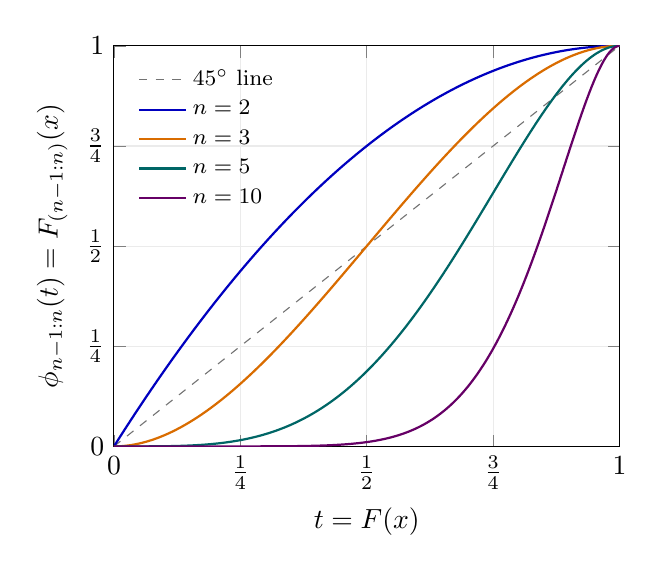
\begin{tikzpicture}
    \begin{axis}[
      width=0.66\textwidth, height=0.55\textwidth,
      xmin=0, xmax=1, ymin=0, ymax=1,
      xlabel={$t = F(x)$},
      ylabel={$\phi_{n-1:n}(t) = F_{(n-1:n)}(x)$},
      xtick={0,0.25,0.5,0.75,1}, ytick={0,0.25,0.5,0.75,1},
      xticklabels={$0$,$\frac{1}{4}$,$\frac{1}{2}$,$\frac{3}{4}$,$1$},
      yticklabels={$0$,$\frac{1}{4}$,$\frac{1}{2}$,$\frac{3}{4}$,$1$},
      grid=major, grid style={black!8},
      legend style={at={(0.03,0.97)}, anchor=north west, font=\footnotesize, draw=none, fill=none},
      legend cell align=left,
      samples=200, domain=0:1,
    ]
      \addplot[black!55, dashed, thin] {x};
      \addlegendentry{$45^\circ$ line}
      \addplot[blue!75!black, thick] {2*x - x^2};
      \addlegendentry{$n = 2$}
      \addplot[orange!85!black, thick] {3*x^2 - 2*x^3};
      \addlegendentry{$n = 3$}
      \addplot[teal!80!black, thick] {5*x^4 - 4*x^5};
      \addlegendentry{$n = 5$}
      \addplot[violet!80!black, thick] {10*x^9 - 9*x^10};
      \addlegendentry{$n = 10$}
    \end{axis}
  \end{tikzpicture}
  \caption{The map $\phi_{n-1:n}(t) = nt^{n-1} - (n-1)t^n$ from the parent CDF to the CDF of the
  second-highest of $n$ draws, for $n = 2, 3, 5, 10$. Each map is a strictly increasing bijection of
  $[0,1]$, so it can be inverted (\cref{prop:B-os-identification}). Every map is flat at $t = 1$, and for $n
  \geq 3$ it is also flat near $t = 0$ over a range that widens with $n$. Where the map is flat, small errors
  in the price distribution become large errors in $F$, so the tails of $F$ are hard to recover from
  transaction prices (\cref{rem:B-os-precision}).}
  \label{fig:B-ordermap}
\end{figure}

\begin{example}[First-price auctions with only the winning bid]\label{ex:B-os-winning-bid}
In a first-price auction with symmetric independent private values, equilibrium bids are i.i.d.\ with some
CDF $G$ and density $g$. A Dutch auction records only the winning bid $B_{(n:n)}$, whose CDF is $G^n$ and
whose density is $nG^{n-1}g$. Hence
\begin{equation*}
  \frac{G_{(n:n)}(b)}{g_{(n:n)}(b)} = \frac{G(b)^n}{nG(b)^{n-1}g(b)} = \frac{G(b)}{n\,g(b)}.
\end{equation*}
The first-order condition of a bidder delivers the inverse bid function of \citet{GuerrePerrigneVuong2000},
which can be rewritten in terms of the winning-bid distribution:
\begin{equation*}
  v = b + \frac{G(b)}{(n-1)g(b)} = b + \frac{n}{n-1}\cdot\frac{G_{(n:n)}(b)}{g_{(n:n)}(b)}.
\end{equation*}
The value distribution is therefore identified from winning bids alone when $n$ is known
\citep[Section~3.3.1, eq.~(3.7)]{AtheyHaile2007}. \Cref{ch:auction-empirics} develops the inversion.
\end{example}

Without symmetry, the parent distributions differ across bidders and one order statistic cannot separate
them. Observing the identity of the winner restores identification. The argument comes from the
statistics of \emph{competing risks}, where a system fails when its first component fails and we observe the
failure time and which component failed \citep{Berman1963}. Up to a sign change, this is the same as
observing the highest bid and the identity of the highest bidder \citep[fn.~21]{AtheyHaile2002}.

\begin{proposition}[Competing risks]\label{prop:B-competing-risks}
Let $X_1, \dots, X_n$ be independent, with continuous CDFs $F_1, \dots, F_n$ that share the support
$[\underline x, \bar x]$. Suppose we observe the maximum $M = \max_i X_i$ and the identity $I$ of the
maximizer. Define $G_i^w(x) = \Pr(M \leq x, I = i)$. Then each $F_i$ is identified, and for every $x$ in the
interior of the support
\begin{equation}\label{eq:B-competing-risks}
  F_i(x) = \exp\left(-\int_x^{\bar x}\frac{\dd G_i^w(t)}{\sum_{j=1}^{n}G_j^w(t)}\right).
\end{equation}
\end{proposition}

\begin{proof}
For transparency we assume densities $f_i$. The general case replaces $f_i(t)\,\dd t$ by $\dd F_i(t)$.

\emph{Step 1.} Bidder $i$ wins with a value at most $x$ when $X_i \leq x$ and every rival draw is below
$X_i$. Conditioning on $X_i = t$ and using independence,
\begin{equation*}
  G_i^w(x) = \Pr\big(X_i \leq x,\ X_j < X_i \ \forall j \neq i\big) = \int_{\underline x}^{x}
  \prod_{j \neq i}F_j(t)\,f_i(t)\,\dd t.
\end{equation*}

\emph{Step 2.} Ties have probability zero, so the events $\{I = j\}$ partition the sample space. Summing over
$j$ gives the CDF of the maximum:
\begin{equation*}
  \sum_{j=1}^{n}G_j^w(x) = \Pr(M \leq x) = \prod_{j=1}^{n}F_j(x) \equiv F_M(x).
\end{equation*}

\emph{Step 3.} For $t$ in the interior of the support, $F_i(t) > 0$. Writing the integrand of Step 1 as
$\frac{F_M(t)}{F_i(t)}f_i(t)$,
\begin{equation*}
  \dd G_i^w(t) = F_M(t)\,\frac{f_i(t)}{F_i(t)}\,\dd t = F_M(t)\,\dd\ln F_i(t).
\end{equation*}

\emph{Step 4.} Divide by $F_M(t)$, which is positive on the interior because the supports coincide, and
integrate from $x$ to $\bar x$:
\begin{equation*}
  \int_x^{\bar x}\frac{\dd G_i^w(t)}{F_M(t)} = \ln F_i(\bar x) - \ln F_i(x) = -\ln F_i(x).
\end{equation*}
Exponentiating and substituting Step 2 for $F_M$ gives \eqref{eq:B-competing-risks}. Every term on the right
is a feature of the distribution of $(M, I)$.
\end{proof}

\Citet[Theorem~2]{AtheyHaile2002} state this result for asymmetric independent private values. Their case
(b) observes the highest bid of a second-price auction together with the winner's identity, which is
\cref{prop:B-competing-risks}. Their case (a) observes the transaction price $X_{(n-1:n)}$ and the winner's
identity, and identification then follows from \citet{Meilijson1981}. We omit that more involved argument.
\citet[Section~3.3.1, eq.~(3.8)]{AtheyHaile2007} apply \eqref{eq:B-competing-risks} to the winning bid and
winner's identity in a first-price auction. This identifies each bidder's bid distribution, and the
first-order conditions then identify the value distributions. The common support matters. If some rival's
values never fall below $a$, bidder $i$ never wins with a value below $a$, so $F_i$ is not identified there.
Theorem~2 relaxes symmetry and keeps independence. Dropping independence as well destroys point
identification, a classic result for competing risks \citep{Tsiatis1975}. \Citet[Theorem~2, p.~2116]{AtheyHaile2002}
also give two routes to testing the model. In the first, participation is exogenous and each bidder faces at
least two different sets of opponents. Each set identifies $F_i$, and the versions must agree. In the second, a
second-price auction reveals both the transaction price and the highest bid, each with the winner's identity.
Cases (a) and (b) then deliver two versions of $F_i$, which again must coincide.

\begin{remark}[Minima and procurement]\label{rem:B-competing-min}
In a procurement auction we observe the lowest cost $m = \min_i X_i$ and the identity of the low bidder. The
mirror image of the proof uses $G_i^\ell(x) = \Pr(m \leq x, I = i) = \int_{\underline x}^{x}\prod_{j \neq
i}[1 - F_j(t)]\,\dd F_i(t)$ and the survival function of the minimum, $S_m(t) = \prod_j[1 - F_j(t)] = 1 -
\sum_jG_j^\ell(t)$. Then $\dd G_i^\ell(t) = -S_m(t)\,\dd\ln[1 - F_i(t)]$, and integrating from $\underline x$
to $x$ gives
\begin{equation*}
  1 - F_i(x) = \exp\left(-\int_{\underline x}^{x}\frac{\dd G_i^\ell(t)}{1 - \sum_{j=1}^{n}G_j^\ell(t)}\right).
\end{equation*}
The integrand is the \emph{cause-specific hazard} of reliability theory.
\end{remark}

\begin{example}[Two exponential suppliers]\label{ex:B-competing-exp}
Let supplier $i \in \{1, 2\}$ have cost $X_i$ with $F_i(x) = 1 - e^{-\lambda_ix}$ on $[0, \infty)$, where the
rates $\lambda_i > 0$ are local notation. The probability that supplier 1 wins at a cost at most $x$ is
\begin{equation*}
  G_1^\ell(x) = \int_0^x e^{-\lambda_2t}\lambda_1e^{-\lambda_1t}\,\dd t
  = \frac{\lambda_1}{\lambda_1 + \lambda_2}\Big(1 - e^{-(\lambda_1 + \lambda_2)x}\Big).
\end{equation*}
The minimum has survival function $S_m(t) = e^{-(\lambda_1 + \lambda_2)t}$. Hence $\frac{\dd
G_1^\ell(t)}{S_m(t)} = \lambda_1\,\dd t$, and the formula of \cref{rem:B-competing-min} returns $1 - F_1(x) =
e^{-\lambda_1x}$. The example shows where the information comes from. The winning cost is exponential with
rate $\lambda_1 + \lambda_2$ whoever wins, and the frequency with which supplier 1 wins, $\frac{\lambda_1}
{\lambda_1 + \lambda_2}$, splits the total rate between the two suppliers.
\end{example}

\subsection{Deconvolution and Kotlarski's lemma}\label{sec:B-kotlarski}

A related tool separates a common component from idiosyncratic ones. It is used for auctions with
unobserved heterogeneity, where all bids in an auction share a component that the econometrician does not
observe. We write $\mathrm{i}$ for the imaginary unit and $\psi_X(t) = \E[e^{\mathrm{i}tX}]$ for the
\emph{characteristic function} of a random variable $X$.

\begin{lemma}[Kotlarski]\label{lem:B-kotlarski}
Let $Y_1, Y_2, Y_3$ be mutually independent with nonvanishing characteristic functions. Assume $\E|Y_1| <
\infty$ and $\E|Y_3| < \infty$, and normalize $\E[Y_1] = 0$. Let $Q_1 = Y_1 + Y_3$ and $Q_2 = Y_2 + Y_3$, with
joint characteristic function $\psi_Q(t_1, t_2) = \E[e^{\mathrm{i}(t_1Q_1 + t_2Q_2)}]$, and let $\partial_1$
denote the derivative with respect to the first argument. Then the distribution of $(Q_1, Q_2)$ determines
the distributions of $Y_1$, $Y_2$ and $Y_3$, through
\begin{equation}\label{eq:B-kotlarski}
  \psi_{Y_3}(t) = \exp\left(\int_0^t\frac{\partial_1\psi_Q(0, u)}{\psi_Q(0, u)}\,\dd u\right), \qquad
  \psi_{Y_1}(t) = \frac{\psi_Q(t, 0)}{\psi_{Y_3}(t)}, \qquad
  \psi_{Y_2}(t) = \frac{\psi_Q(0, t)}{\psi_{Y_3}(t)}.
\end{equation}
\end{lemma}

\begin{proof}
\emph{Step 1 (factorization).} Write $t_1Q_1 + t_2Q_2 = t_1Y_1 + t_2Y_2 + (t_1 + t_2)Y_3$. Independence gives
\begin{equation*}
  \psi_Q(t_1, t_2) = \psi_{Y_1}(t_1)\,\psi_{Y_2}(t_2)\,\psi_{Y_3}(t_1 + t_2).
\end{equation*}

\emph{Step 2 (differentiation).} The moment conditions make $\psi_{Y_1}$ and $\psi_{Y_3}$ differentiable, with
$\psi_{Y_1}'(0) = \mathrm{i}\E[Y_1] = 0$ and $\psi_{Y_1}(0) = 1$. Differentiating Step 1 in $t_1$ at $t_1 = 0$,
\begin{equation*}
  \partial_1\psi_Q(0, u) = \psi_{Y_1}'(0)\psi_{Y_2}(u)\psi_{Y_3}(u) + \psi_{Y_2}(u)\psi_{Y_3}'(u)
  = \psi_{Y_2}(u)\psi_{Y_3}'(u).
\end{equation*}
Since $\psi_Q(0, u) = \psi_{Y_2}(u)\psi_{Y_3}(u)$ and the characteristic functions do not vanish,
\begin{equation*}
  \frac{\partial_1\psi_Q(0, u)}{\psi_Q(0, u)} = \frac{\psi_{Y_3}'(u)}{\psi_{Y_3}(u)}.
\end{equation*}

\emph{Step 3 (integration).} Let $\ell(t) = \int_0^t\frac{\psi_{Y_3}'(u)}{\psi_{Y_3}(u)}\,\dd u$ and $h(t) =
\psi_{Y_3}(t)e^{-\ell(t)}$. Then $h'(t) = \psi_{Y_3}'(t)e^{-\ell(t)} - \psi_{Y_3}(t)\ell'(t)e^{-\ell(t)} = 0$, and
$h(0) = 1$. So $h \equiv 1$, which is the first formula in \eqref{eq:B-kotlarski}. Setting $t_2 = 0$ or $t_1 =
0$ in Step 1 gives the other two. A characteristic function determines its distribution, which completes the
proof.
\end{proof}

The lemma is Lemma~6.1 of \citet{AtheyHaile2007}, after \citet{Kotlarski1966} and \citet{PrakasaRao1992}.
\Cref{lem:15-kotlarski} gives the same result in auction notation, together with identification up to location
when the mean of $Y_1$ is unknown. The normalization is needed because adding a constant to $Y_3$ and subtracting it from $Y_1$ and $Y_2$ leaves
$(Q_1, Q_2)$ unchanged. In auctions with additive unobserved heterogeneity, a bidder's value is
$A_{it} + V_{0t}$, where $V_{0t}$ is common to auction $t$ and unobserved. Equilibrium bids then take the form
$B_{it} = B^0_{it} + V_{0t}$, where the homogenized bid $B^0_{it}$ is the bid in an auction with $V_{0t} = 0$
\citep[Section~6.1.2]{AtheyHaile2007}. Two bids from the same auction play the roles of $Q_1$ and $Q_2$, with
$Y_3 = V_{0t}$. \Cref{lem:B-kotlarski} recovers the distribution of homogenized bids, and the first-order
condition then recovers values. \citet{Krasnokutskaya2011} uses the multiplicative version, which becomes
additive after taking logarithms (\cref{ch:auction-empirics}).

\section{Fixed points and the contraction mapping theorem}\label{sec:B-fixedpoint}

Many objects in industrial organization are \emph{fixed points}, points $x^*$ with $\Phi(x^*) = x^*$ for some
map $\Phi$. The mean utilities that rationalize observed shares solve $\delta = \delta + \ln s^{obs} - \ln
s(\delta)$. Equilibrium prices solve $p = BR(p)$, where $BR$ stacks the firms' best responses. Value
functions of dynamic problems solve Bellman equations. Each case raises three questions. Does a fixed point
exist? Is it unique? How do we compute it? The contraction mapping theorem answers all three at once when it
applies. Brouwer's and Kakutani's theorems answer only the first, and uniqueness then needs a separate
argument such as diagonal dominance. The proof of the implicit function theorem (\cref{thm:B-ift}) already
relied on the contraction mapping theorem, which we now prove. Throughout, $\Phi$ is the map, $\kappa \in [0,1)$
a modulus, $x^*$ a fixed point and $x^{(h)}$ the $h$-th iterate.

\subsection{Metric spaces and contractions}\label{sec:B-metric}

\begin{definition}[Metric space]\label{def:B-metric}
A \emph{metric space} is a set $X$ with a function $d: X \times X \to [0, \infty)$ with three properties
for all $x, y, z \in X$.
\begin{enumerate}[label=(\roman*)]
  \item $d(x, y) = 0$ if and only if $x = y$.
  \item $d(x, y) = d(y, x)$.
  \item $d(x, z) \leq d(x, y) + d(y, z)$.
\end{enumerate}
A sequence $(x^{(h)})$ is \emph{Cauchy} if for every $\epsilon > 0$ there is $H$ with $d(x^{(h)},
x^{(m)}) < \epsilon$ for all $h, m \geq H$. The space is \emph{complete} if every Cauchy sequence converges
to a point of $X$.
\end{definition}

The leading example is $\R^n$ with the sup norm $\|x\|_\infty = \max_k |x_k|$ and $d(x, y) = \|x -
y\|_\infty$. A sequence that is Cauchy in this metric is Cauchy coordinate by coordinate, and $\R$ is
complete, so $(\R^n, \|\cdot\|_\infty)$ is complete. A closed subset of a complete space is complete, because
limits of its sequences stay in the set. Boxes $[\underline y, \bar y]^J$ and orthants $(-\infty, \bar
\delta]^J$ are therefore complete. The interval $(0, 1]$ is not complete, since the Cauchy sequence
$\frac{1}{h}$ converges to $0 \notin (0,1]$. The set of bounded real functions on a set $S$, with the metric
$\sup_{s \in S}|g(s) - g'(s)|$, is complete. So is its subset of bounded continuous functions when $S$ is a
metric space \citep{StokeyLucas1989}. Dynamic programming works in these function spaces.

\begin{definition}[Contraction]\label{def:B-contraction}
A map $\Phi: X \to X$ is a \emph{contraction with modulus} $\kappa \in [0,1)$ if
\begin{equation*}
  d\big(\Phi(x), \Phi(y)\big) \leq \kappa\, d(x, y) \qquad \text{for all } x, y \in X.
\end{equation*}
\end{definition}

A map that satisfies the inequality with some $\kappa \geq 0$ is \emph{Lipschitz} with constant $\kappa$. A
contraction is Lipschitz and hence continuous. The uniform modulus is essential. Consider $\Phi(x) = x +
\frac{1}{x}$ on $[1, \infty)$. It maps the set into $[2, \infty)$, and $\Phi'(x) = 1 - \frac{1}{x^2} \in [0,
1)$, so the mean value theorem gives $|\Phi(x) - \Phi(y)| < |x - y|$ whenever $x \neq y$. Yet $\Phi(x) = x$
would require $\frac{1}{x} = 0$, so there is no fixed point. The local modulus $\Phi'(x)$ approaches one as $x
\to \infty$, and the iterates drift off to infinity. The share inversion has the same feature, which is why
\citet{BerryLevinsohnPakes1995} truncate the map (\cref{thm:B-blp-contraction}). Completeness matters too.
The map $\Phi(x) = \frac{x}{2}$ is a contraction of $(0,1]$ into itself without a fixed point in $(0,1]$.

\subsection{The Banach fixed-point theorem}\label{sec:B-banach}

\begin{theorem}[Banach fixed-point theorem]\label{thm:B-banach}
Let $(X, d)$ be a complete metric space and let $\Phi: X \to X$ be a contraction with modulus $\kappa$. Then
the following hold.
\begin{enumerate}[label=(\roman*)]
  \item $\Phi$ has exactly one fixed point $x^*$.
  \item For every starting point $x^{(0)} \in X$, the iterates $x^{(h+1)} = \Phi(x^{(h)})$ converge to $x^*$.
  \item $d(x^{(h)}, x^*) \leq \kappa^h\,d(x^{(0)}, x^*)$ for all $h$.
\end{enumerate}
\end{theorem}

\begin{proof}
\emph{Step 1 (successive steps shrink geometrically).} For $h \geq 1$,
\begin{equation*}
  d\big(x^{(h+1)}, x^{(h)}\big) = d\big(\Phi(x^{(h)}), \Phi(x^{(h-1)})\big) \leq \kappa\,d\big(x^{(h)},
  x^{(h-1)}\big).
\end{equation*}
Applying this $h$ times gives $d(x^{(h+1)}, x^{(h)}) \leq \kappa^h d_0$, where $d_0 = d(x^{(1)}, x^{(0)})$.

\emph{Step 2 (the iterates form a Cauchy sequence).} For $m > h$, the triangle inequality and Step 1 give
\begin{equation*}
  d\big(x^{(m)}, x^{(h)}\big) \leq \sum_{l=h}^{m-1}d\big(x^{(l+1)}, x^{(l)}\big) \leq d_0\sum_{l=h}^{m-1}
  \kappa^l \leq \frac{\kappa^h}{1 - \kappa}\,d_0.
\end{equation*}
The bound tends to zero as $h \to \infty$, so the sequence is Cauchy. By completeness it converges to some
$x^* \in X$.

\emph{Step 3 (the limit is a fixed point).} For every $h$,
\begin{equation*}
  d\big(\Phi(x^*), x^*\big) \leq d\big(\Phi(x^*), \Phi(x^{(h)})\big) + d\big(x^{(h+1)}, x^*\big)
  \leq \kappa\,d\big(x^*, x^{(h)}\big) + d\big(x^{(h+1)}, x^*\big).
\end{equation*}
The right side tends to zero, so $\Phi(x^*) = x^*$.

\emph{Step 4 (uniqueness).} If $\Phi(y) = y$, then $d(x^*, y) = d(\Phi(x^*), \Phi(y)) \leq \kappa\,d(x^*, y)$.
Since $\kappa < 1$, this forces $d(x^*, y) = 0$.

\emph{Step 5 (the rate).} $d(x^{(h)}, x^*) = d(\Phi(x^{(h-1)}), \Phi(x^*)) \leq \kappa\,d(x^{(h-1)}, x^*)$, and
induction gives (iii).
\end{proof}

The theorem is due to \citet{Banach1922}. Part (iii) says that the error falls at least geometrically, a
property called \emph{linear convergence}. In practice we do not know $x^*$, so we need bounds in terms of
computable quantities.

\begin{corollary}[Error bounds]\label{cor:B-banach-bounds}
Under the conditions of \cref{thm:B-banach}, for every $h \geq 1$,
\begin{align}
  d\big(x^{(h)}, x^*\big) &\leq \frac{\kappa^h}{1 - \kappa}\,d\big(x^{(1)}, x^{(0)}\big)
  && \text{(a priori bound)}, \label{eq:B-apriori}\\
  d\big(x^{(h)}, x^*\big) &\leq \frac{\kappa}{1 - \kappa}\,d\big(x^{(h)}, x^{(h-1)}\big)
  && \text{(a posteriori bound)}. \label{eq:B-aposteriori}
\end{align}
\end{corollary}

\begin{proof}
For \eqref{eq:B-apriori}, let $m \to \infty$ in Step 2 of the proof of \cref{thm:B-banach}, using continuity
of $d$. For \eqref{eq:B-aposteriori}, apply the triangle inequality and the contraction property:
\begin{align*}
  d\big(x^{(h)}, x^*\big) &= d\big(\Phi(x^{(h-1)}), \Phi(x^*)\big) \leq \kappa\,d\big(x^{(h-1)}, x^*\big) \\
  &\leq \kappa\,d\big(x^{(h-1)}, x^{(h)}\big) + \kappa\,d\big(x^{(h)}, x^*\big).
\end{align*}
Collecting the terms in $d(x^{(h)}, x^*)$ gives $(1 - \kappa)\,d(x^{(h)}, x^*) \leq \kappa\,d(x^{(h)},
x^{(h-1)})$.
\end{proof}

The a posteriori bound justifies the usual stopping rule, which halts when successive iterates are within
a tolerance $\varepsilon_{tol}$. The rule controls the true error only up to the factor $\frac{\kappa}{1 -
\kappa}$. This factor is 1 for $\kappa = \frac{1}{2}$, 9 for $\kappa = 0.9$ and 99 for $\kappa = 0.99$, so the
stopping tolerance must be tighter than the accuracy we want when $\kappa$ is near one.
\Cref{prop:08-innererror} applies this bound to the inner loop of BLP estimation. The a priori bound tells us
how many iterations suffice. The bound is below $\varepsilon_{tol}$ when $\kappa^h d(x^{(1)}, x^{(0)}) \leq
\varepsilon_{tol}(1 - \kappa)$. Taking logarithms and dividing by $\ln\kappa < 0$, which reverses the
inequality,
\begin{equation}\label{eq:B-iterations}
  h \geq \frac{\ln\big(\varepsilon_{tol}(1 - \kappa)\big) - \ln d\big(x^{(1)}, x^{(0)}\big)}{\ln\kappa}.
\end{equation}
With $d(x^{(1)}, x^{(0)}) = 1$ and $\varepsilon_{tol} = 10^{-12}$, the bound requires 41 iterations for $\kappa =
\frac{1}{2}$, 285 for $\kappa = 0.9$ and 3,208 for $\kappa = 0.99$. The cost of a fixed-point computation grows
roughly like $\frac{1}{1 - \kappa}$.

\begin{remark}[Contractions on subsets]\label{rem:B-local-contraction}
The theorem applies to any closed subset $C \subseteq X$ that $\Phi$ maps into itself and on which $\Phi$
contracts, since $C$ is complete. A convenient sufficient condition uses a closed ball. Suppose $\Phi$ is
Lipschitz with constant $\kappa < 1$ on $\bar B = \{x : d(x, x^{(0)}) \leq \tau\}$ and $d(\Phi(x^{(0)}),
x^{(0)}) \leq (1 - \kappa)\tau$. Then for $x \in \bar B$,
\begin{equation*}
  d\big(\Phi(x), x^{(0)}\big) \leq d\big(\Phi(x), \Phi(x^{(0)})\big) + d\big(\Phi(x^{(0)}), x^{(0)}\big)
  \leq \kappa\tau + (1 - \kappa)\tau = \tau,
\end{equation*}
so $\Phi$ maps $\bar B$ into itself and has a unique fixed point there. The proof of the implicit function
theorem (\cref{thm:B-ift}) uses this device, and so does the truncation argument of
\cref{thm:B-blp-contraction}.
\end{remark}

\begin{remark}[Local convergence and the choice of norm]\label{rem:B-ostrowski}
Suppose $\Phi: \R^n \to \R^n$ is continuously differentiable near a fixed point $x^*$. If the spectral radius
of the Jacobian $D\Phi(x^*)$, the largest modulus of its eigenvalues, is below one, then the iterates
converge to $x^*$ from every starting point close enough to it. The asymptotic rate equals the spectral
radius. If some eigenvalue has modulus above one, $x^*$ repels the iterates in the direction of the
corresponding eigenvector, and iteration started near $x^*$ generally fails to converge \citep{Judd1998}.
The contraction property depends on the metric. The matrix $A = \begin{psmallmatrix}0 & 2\\ 0 &
0\end{psmallmatrix}$ has spectral radius zero, and $A^2x = 0$ for every $x$, yet $\|Ax\|_\infty = 2\|x\|_\infty$
for $x = (0, 1)$. The sup norm suits the applications below because row sums of Jacobians are easy to bound.
\end{remark}

\Cref{fig:B-cobweb} shows the iteration on the real line as a \emph{cobweb}. Each step moves vertically to
the graph of $\Phi$ and then horizontally to the 45-degree line. In the left panel, $\Phi(x) = 1 +
\frac{1}{2}\cos x$ has $|\Phi'(x)| = \frac{1}{2}|\sin x| \leq \frac{1}{2}$, so it is a contraction of $\R$ with
modulus $\frac{1}{2}$. Starting from $x^{(0)} = 0$, the iterates are $1.5$, $1.035$, $1.255$, $1.155$ and so on,
and they converge to $x^* = 1.187151$. After ten steps the error is $3.2 \times 10^{-4}$, below the a priori
bound $\frac{\kappa^{10}}{1 - \kappa}\,d(x^{(1)}, x^{(0)}) = 2^{-9} \times 1.5 = 2.9 \times 10^{-3}$. The errors shrink by a factor close to
$|\Phi'(x^*)| = 0.464$ per step, as \cref{rem:B-ostrowski} predicts. In the right panel, $\Phi(x) = 3 -
\frac{3}{2}x$ has slope $-\frac{3}{2}$. Its fixed point is $x^* = \frac{6}{5}$, but from $x^{(0)} = 1$ the
distance to $x^*$ grows by the factor $\frac{3}{2}$ each step, from $0.2$ to $0.3$, $0.45$, $0.675$ and
beyond. The negative slope makes the path spiral, and the slope above one in absolute value makes it diverge.

\begin{figure}[htbp]
  \centering
  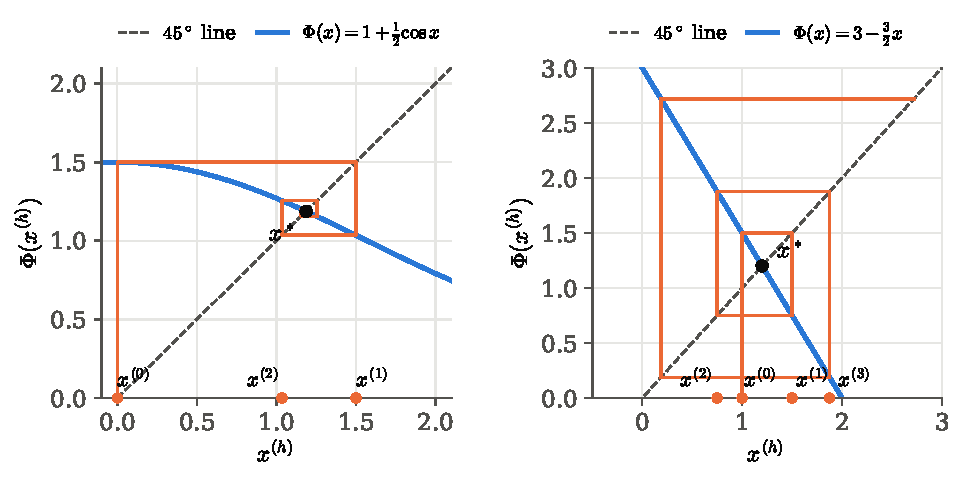
\includegraphics[width=0.95\textwidth]{figures/appB/cobweb.pdf}
  \caption{Cobweb diagrams for the iteration $x^{(h+1)} = \Phi(x^{(h)})$. In the left panel, $\Phi(x) = 1 +
  \frac{1}{2}\cos x$ is a contraction with modulus $\frac{1}{2}$, and the path from $x^{(0)} = 0$ converges to
  the fixed point $x^* \approx 1.187$. In the right panel, $\Phi(x) = 3 - \frac{3}{2}x$ has slope $-\frac{3}{2}$, and the path
  from $x^{(0)} = 1$ spirals away from the fixed point $x^* = \frac{6}{5}$.}
  \label{fig:B-cobweb}
\end{figure}

\subsection{Checking the contraction property}\label{sec:B-contraction-criteria}

For smooth maps on $\R^n$, the contraction property follows from a bound on the Jacobian.

\begin{proposition}[Jacobian row-sum criterion]\label{prop:B-jacobian-criterion}
Let $X \subseteq \R^n$ be convex and let $\Phi: X \to \R^n$ be continuously differentiable on an open set
containing $X$. If
\begin{equation}\label{eq:B-rowsum-criterion}
  \sup_{x \in X}\ \max_{j}\sum_{k=1}^{n}\left|\frac{\partial\Phi_j(x)}{\partial x_k}\right| \leq \kappa,
\end{equation}
then $\|\Phi(x) - \Phi(y)\|_\infty \leq \kappa\|x - y\|_\infty$ for all $x, y \in X$. If in addition $\kappa < 1$
and $\Phi$ maps $X$ into itself, then $\Phi$ is a contraction of $X$ in the sup norm.
\end{proposition}

\begin{proof}
Fix $x, y \in X$ and a component $j$. By convexity the segment $x + \tau(y - x)$, $\tau \in [0,1]$, lies in
$X$. The fundamental theorem of calculus and the chain rule give
\begin{equation*}
  \Phi_j(y) - \Phi_j(x) = \int_0^1\sum_{k=1}^{n}\frac{\partial\Phi_j}{\partial x_k}\big(x + \tau(y -
  x)\big)\,(y_k - x_k)\,\dd\tau.
\end{equation*}
Bounding each $|y_k - x_k|$ by $\|y - x\|_\infty$,
\begin{equation*}
  |\Phi_j(y) - \Phi_j(x)| \leq \int_0^1\sum_{k=1}^{n}\left|\frac{\partial\Phi_j}{\partial x_k}\big(x +
  \tau(y - x)\big)\right|\,\dd\tau\ \|y - x\|_\infty \leq \kappa\|y - x\|_\infty.
\end{equation*}
Taking the maximum over $j$ proves the claim.
\end{proof}

The constant in \eqref{eq:B-rowsum-criterion} is the largest induced sup norm of the Jacobian over $X$, by
\cref{lem:B-rowsum}. For a linear map the criterion is therefore sharp. The proof is the mean value
inequality of \cref{sec:B-calculus}.

When all partial derivatives are nonnegative, as in the share inversion below, the absolute values in
\eqref{eq:B-rowsum-criterion} drop out. The row sum then has a direct reading:
\begin{equation*}
  \sum_{k=1}^{n}\frac{\partial\Phi_j(x)}{\partial x_k} = \frac{\dd}{\dd c}\,\Phi_j(x + c\mathbf{1})\Big|_{c=0},
\end{equation*}
where $\mathbf{1}$ is the vector of ones. The condition says that $\Phi$ is monotone and that raising every
argument by $c$ raises each component by less than $c$. Blackwell's theorem is the version of this idea for
maps between function spaces.

\begin{theorem}[\citealp{Blackwell1965}]\label{thm:B-blackwell}
Let $B(S)$ be the space of bounded real functions on a set $S$ with the sup metric, and let $\mathcal{T}:
B(S) \to B(S)$ satisfy two conditions. The first, monotonicity, requires that $g \leq g'$ pointwise implies
$\mathcal{T}g \leq \mathcal{T}g'$. The second, discounting, requires that there is $\kappa \in [0,1)$ such that $\mathcal{T}(g + c) \leq \mathcal{T}g +
\kappa c$ for every $g$ and every constant $c \geq 0$. Then $\mathcal{T}$ is a contraction with modulus $\kappa$.
\end{theorem}

\begin{proof}
Fix $g, g' \in B(S)$ and let $c = \sup_s|g(s) - g'(s)|$. Then $g \leq g' + c$ pointwise. Monotonicity and
discounting give $\mathcal{T}g \leq \mathcal{T}(g' + c) \leq \mathcal{T}g' + \kappa c$. Exchanging the roles
of $g$ and $g'$ gives $\mathcal{T}g' \leq \mathcal{T}g + \kappa c$. Hence $|\mathcal{T}g(s) - \mathcal{T}g'(s)|
\leq \kappa c$ for every $s$, which is the claim.
\end{proof}

The Bellman operator $(\mathcal{T}g)(s) = \max_a\{u(s, a) + \kappa\,\E[g(s') \mid s, a]\}$ of a dynamic program
with discount factor $\kappa$ satisfies both conditions, so value functions are unique fixed points that
value iteration computes. Dynamic models lie outside this edition, but the logic is the same as in the
static applications below.

Some maps of interest have row sums below one at every point but not uniformly, as in the example $x +
\frac{1}{x}$. \Citet[Appendix~I]{BerryLevinsohnPakes1995} handle this case with a truncation.

\begin{theorem}[\citealp{BerryLevinsohnPakes1995}, Appendix I]\label{thm:B-blp-contraction}
Consider $\R^J$ with the sup norm, and let $\Phi: \R^J \to \R^J$ satisfy three conditions. (1) $\Phi$ is
continuously differentiable, with $\frac{\partial\Phi_j(y)}{\partial y_k} \geq 0$ and $\sum_{k=1}^{J}
\frac{\partial\Phi_j(y)}{\partial y_k} < 1$ for all $j$, $k$ and $y$. (2) $\Phi$ is bounded below:
$\underline y \equiv \min_j\inf_y\Phi_j(y) > -\infty$. (3) There is a value $\bar y$ such that, whenever $y_j
\geq \bar y$ for some $j$, there is some $k$ (not necessarily equal to $j$) with $\Phi_k(y) < y_k$. Then
$\Phi$ has a unique fixed point in $\R^J$. Moreover, the truncated map $\hat\Phi_j(y) = \min\{\Phi_j(y),
\bar y\}$ is a contraction of $[\underline y, \bar y]^J$ with modulus below one.
\end{theorem}

\Cref{thm:08-contraction} proves the theorem in full. The idea is short. On the compact set $[\underline y,
\bar y]^J$, enlarged by the segments along which the proof integrates, the continuous row sums attain a
maximum $\kappa < 1$. The truncated map is therefore a contraction there, and \cref{thm:B-banach} gives a
fixed point. Condition (3) keeps that fixed point away from the cap $\bar y$, so it is a fixed point of
$\Phi$ itself. The bound $\bar y$ is needed because no uniform modulus exists on all of $\R^J$. In the logit
model, for instance, the row sums of the share-inversion map equal $1 - s_0(\delta)$, which tends to one as
the mean utilities grow (\cref{sec:B-inversion}).

\subsection{Application: inverting market shares}\label{sec:B-inversion}

Consider a market with inside goods $j = 1, \dots, J$ and the outside good $j = 0$. In the random
coefficients logit model, consumer $i$ chooses $j$ with probability
\begin{equation*}
  s_{ij}(\delta) = \frac{e^{\delta_j + \mu_{ij}}}{1 + \sum_{k=1}^{J}e^{\delta_k + \mu_{ik}}}, \qquad
  s_{i0}(\delta) = 1 - \sum_{k=1}^{J}s_{ik}(\delta),
\end{equation*}
and the market share is $s_j(\delta) = \int s_{ij}(\delta)\,\dd F(\nu_i)$, where $\mu_{ij}$ depends on the
consumer's tastes $\nu_i$ and the nonlinear parameters (\cref{ch:blp}). Given observed shares $s^{obs}$
with $s^{obs}_j > 0$ and $\sum_js^{obs}_j < 1$, estimation needs the vector $\delta$ that solves $s(\delta) =
s^{obs}$. \citet[eq.~(6.8), p.~865]{BerryLevinsohnPakes1995} compute it as the fixed point of
\begin{equation}\label{eq:B-blp-map}
  \Phi_j(\delta) = \delta_j + \ln s^{obs}_j - \ln s_j(\delta), \qquad j = 1, \dots, J.
\end{equation}
A vector $\delta$ is a fixed point of $\Phi$ exactly when $s(\delta) = s^{obs}$.

\begin{proposition}[Row sums of the BLP map]\label{prop:B-blp-rowsum}
In the random coefficients logit model, for all $j$ and all $k \neq j$,
\begin{equation*}
  \frac{\partial\Phi_j}{\partial\delta_j} = \frac{1}{s_j}\int s_{ij}^2\,\dd F > 0, \qquad
  \frac{\partial\Phi_j}{\partial\delta_k} = \frac{1}{s_j}\int s_{ij}s_{ik}\,\dd F > 0,
\end{equation*}
and the row sums are
\begin{equation}\label{eq:B-blp-rowsum}
  \sum_{k=1}^{J}\frac{\partial\Phi_j}{\partial\delta_k} = 1 - \frac{1}{s_j}\int s_{ij}s_{i0}\,\dd F \in (0, 1).
\end{equation}
\end{proposition}

\begin{proof}
The individual logit derivatives are $\frac{\partial s_{ij}}{\partial\delta_k} = s_{ij}(\indic\{j = k\} -
s_{ik})$, bounded by one, so we may differentiate under the integral (\cref{sec:B-calculus}). Hence
$\frac{\partial s_j}{\partial\delta_j} = \int s_{ij}(1 - s_{ij})\,\dd F$ and $\frac{\partial
s_j}{\partial\delta_k} = -\int s_{ij}s_{ik}\,\dd F$ for $k \neq j$. Differentiating \eqref{eq:B-blp-map},
\begin{equation*}
  \frac{\partial\Phi_j}{\partial\delta_j} = 1 - \frac{1}{s_j}\int s_{ij}(1 - s_{ij})\,\dd F
  = 1 - \frac{s_j}{s_j} + \frac{1}{s_j}\int s_{ij}^2\,\dd F = \frac{1}{s_j}\int s_{ij}^2\,\dd F,
\end{equation*}
and $\frac{\partial\Phi_j}{\partial\delta_k} = -\frac{1}{s_j}\frac{\partial s_j}{\partial\delta_k} =
\frac{1}{s_j}\int s_{ij}s_{ik}\,\dd F$. For the row sum, consumer $i$'s choice probabilities depend only on
differences of the utilities $(\delta_0 + \mu_{i0}, \dots, \delta_J + \mu_{iJ})$, with $\delta_0 = \mu_{i0} = 0$.
By \cref{cor:B-translation}, $\sum_{k=0}^{J}\frac{\partial s_{ij}}{\partial\delta_k} = 0$, and the outside
derivative is $\frac{\partial s_{ij}}{\partial\delta_0} = -s_{ij}s_{i0}$. Hence $\sum_{k=1}^{J}\frac{\partial
s_{ij}}{\partial\delta_k} = s_{ij}s_{i0}$. Integrating and dividing by $s_j$,
\begin{equation*}
  \sum_{k=1}^{J}\frac{\partial\Phi_j}{\partial\delta_k} = 1 - \frac{1}{s_j}\sum_{k=1}^{J}\frac{\partial
  s_j}{\partial\delta_k} = 1 - \frac{1}{s_j}\int s_{ij}s_{i0}\,\dd F.
\end{equation*}
The integral is positive and smaller than $\int s_{ij}\,\dd F = s_j$, so the row sum lies in $(0,1)$.
\end{proof}

\Cref{cor:08-rowsum} gives the same computation, and \cref{ch:blp} verifies the remaining conditions of
\cref{thm:B-blp-contraction}. The row sum has a useful reading. The weights $\frac{s_{ij}}{s_j}$ form the
distribution of consumer types among the buyers of $j$. The row sum is therefore one minus the average
probability of choosing the outside good among those buyers. The modulus is close to one when the buyers of
some product rarely choose the outside good, and convergence is then slow. The plain logit model shows this in
its simplest form. There $s_{ij} = s_j$, so $\frac{\partial\Phi_j}{\partial\delta_k} = s_k$ for every $k$,
including $k = j$. The Jacobian is the rank-one matrix $\mathbf{1}s^\T$, whose only nonzero eigenvalue is
$s^\T\mathbf{1} = 1 - s_0$. With $s_0 = 0.1$ the iteration gains one digit of accuracy only every 22 steps,
since $\frac{\ln 10}{-\ln 0.9} \approx 21.9$, although the logit inverse $\delta_j = \ln s_j - \ln s_0$ is
available in closed form.

Three practical rules follow. First, the logit inversion $\ln s^{obs}_j - \ln s^{obs}_0$ is a natural
starting value, and inside an estimation routine the solution at the previous parameter value is better.
Second, the stopping tolerance must be tight, by \eqref{eq:B-aposteriori}, because the inversion error
propagates into the estimation objective (\cref{prop:08-innererror}). \citet{DubeFoxSu2012} study how to improve
the numerical performance of random coefficients demand estimation (\cref{ch:blp}).
Third, the update can be written
multiplicatively as $e^{\delta^{(h+1)}_j} = e^{\delta^{(h)}_j}\frac{s^{obs}_j}{s_j(\delta^{(h)})}$. Each step
raises $\delta_j$ when the model underpredicts the share of $j$ and lowers it when the model overpredicts.

\begin{remark}[Where the iteration typically moves from the logit start]\label{rem:B-logit-start}
For a product with a small share, the logistic function $\frac{e^{u}}{1 + e^{u}}$ is convex in the relevant
range of utilities. Random coefficients spread individual utilities around $\delta_j$. By Jensen's
inequality the average choice probability at a given $\delta$ then exceeds the logit probability, so the
model share at the logit starting value typically exceeds the observed share. The iteration then lowers
$\delta_j$, and the recovered mean utilities typically lie below the logit start. The statement describes a
tendency. It is not a theorem, because the denominators of all products move together. \Cref{ch:blp} and \cref{app:problems}
report worked examples.
\end{remark}

\citet[Appendix]{Berry1994} proved existence and uniqueness of the inverse for a broad class of discrete
choice models without the contraction. His argument combines Brouwer's theorem with a diagonal dominance
condition.

\begin{proposition}[\citealp{Berry1994}, Appendix]\label{prop:B-berry-inverse}
Let $s: \R^J \to (0,1)^J$ be the inside shares of a random utility model with $\delta_0 = 0$. Suppose $s$ is
continuously differentiable, and that for all goods $j, k \in \{0, 1, \dots, J\}$ the share of $j$ rises in
$\delta_j$ and falls in $\delta_k$ for $k \neq j$. Suppose also that, for any values of the other inside mean
utilities, finite or $-\infty$, $s_j \to 0$ as $\delta_j \to -\infty$ and $s_j \to 1$ as $\delta_j \to \infty$. Then for every $s^{obs}$ with positive entries and $\sum_j
s^{obs}_j < 1$ there is exactly one $\delta$ with $s(\delta) = s^{obs}$.
\end{proposition}

\begin{proof}[Outline of the proof]
\emph{Step 1 (the element-by-element inverse).} For each $j$, let $r_j(\delta)$ be the value of $\delta_j$
that makes $s_j(\delta_1, \dots, r_j, \dots, \delta_J) = s^{obs}_j$, given the other mean utilities. It exists,
is unique and is continuous, by monotonicity and the limits. It does not depend on $\delta_j$. The implicit
function theorem (\cref{thm:B-ift}) gives, for $k \neq j$,
\begin{equation*}
  \frac{\partial r_j}{\partial\delta_k} = -\left(\frac{\partial s_j}{\partial\delta_j}\right)^{-1}
  \frac{\partial s_j}{\partial\delta_k} > 0.
\end{equation*}
A vector $\delta$ solves $s(\delta) = s^{obs}$ if and only if it is a fixed point of $r = (r_1, \dots, r_J)$.

\emph{Step 2 (a lower bound).} Since $r_j$ rises in every $\delta_k$, it is bounded below by its limit as all
other $\delta_k \to -\infty$. Let $\underline\delta$ be the smallest of these $J$ limits.

\emph{Step 3 (an upper bound).} For each $j$, let $\bar\delta_j$ be the value of $\delta_j$ that sets the
outside share equal to $s^{obs}_0 = 1 - \sum_ks^{obs}_k$ when all other inside $\delta_k$ are $-\infty$. Choose
$\bar\delta > \max_j\bar\delta_j$. Suppose $\delta_j \geq \bar\delta$ for some $j$. Adding products and
raising $\delta_j$ both lower the outside share, so $s_0(\delta) < s^{obs}_0$. The inside shares then sum to
more than $\sum_ks^{obs}_k$, so $s_k(\delta) > s^{obs}_k$ for some $k$. For that $k$, matching the smaller
observed share requires a lower utility, so $r_k(\delta) < \delta_k$.

\emph{Step 4 (existence).} The truncated map $\bar r_j(\delta) = \min\{r_j(\delta), \bar\delta\}$ is continuous
and maps the box $[\underline\delta, \bar\delta]^J$ into itself. Brouwer's theorem (\cref{thm:B-brouwer})
gives a fixed point $\delta^*$. If $\delta^*_j = \bar\delta$ for some $j$, Step 3 gives $k$ with $\bar
r_k(\delta^*) \leq r_k(\delta^*) < \delta^*_k$, a contradiction. So $\delta^*$ lies below the cap and is a fixed
point of $r$.

\emph{Step 5 (uniqueness).} Shares depend only on utility differences, so \cref{cor:B-translation} gives
$\sum_{k=0}^{J}\frac{\partial s_j}{\partial\delta_k} = 0$. All cross derivatives are negative, including the
one with respect to $\delta_0$. Hence
\begin{equation}\label{eq:B-berry-dd}
  \frac{\partial s_j}{\partial\delta_j} = \sum_{k \neq j,\ k \geq 1}\left|\frac{\partial
  s_j}{\partial\delta_k}\right| + \left|\frac{\partial s_j}{\partial\delta_0}\right| > \sum_{k \neq j,\ k \geq
  1}\left|\frac{\partial s_j}{\partial\delta_k}\right|.
\end{equation}
Dividing by $\frac{\partial s_j}{\partial\delta_j}$ shows that the row sums $\sum_k\big|\frac{\partial
r_j}{\partial\delta_k}\big|$ are below one at every point. On the compact box their maximum $\kappa$ is
below one. The truncation is nonexpansive, so \cref{prop:B-jacobian-criterion} makes $\bar r$ a contraction
of the box. Every solution lies in the box by Steps 2 and 3, so the solution is unique.
\end{proof}

Condition \eqref{eq:B-berry-dd} is (A2) in \citet[p.~261]{Berry1994}. It also makes the Jacobian
$\frac{\partial s}{\partial\delta^\T}$ strictly diagonally dominant, hence nonsingular by \cref{lem:B-dd}.
\Citet[p.~260]{Berry1994} notes that a strictly positive and continuous density of the consumer-level
unobservables suffices for his sign conditions. On the same page he states the limit conditions for finite
values of the other mean utilities. We also allow the value $-\infty$, which Steps 2 and 3 of the proof use.

\begin{remark}[Connected substitutes]\label{rem:B-connected-substitutes}
\citet{BerryGandhiHaile2013} replace Berry's sign conditions by a weaker structure. Write $s_j(\delta, p)$
for the demand system and let $\lambda$ stand for either $-p$ or $\delta$. Goods $0, 1, \dots, J$ are
\emph{connected substitutes} in $\lambda$ if two conditions hold \citep[Definition~1,
p.~1759]{BerryHaile2014}. First, $s_k$ is nonincreasing in $\lambda_j$ for all $j > 0$ and $k \neq j$. Second,
for every nonempty set $\mathcal{K} \subseteq \{1, \dots, J\}$, some $k \in \mathcal{K}$ and some good $\ell
\notin \mathcal{K}$ have $s_\ell$ strictly decreasing in $\lambda_k$. The first condition requires weak gross
substitutes. The second requires enough strict substitution that no group of inside goods trades only among
itself, where the outside good may serve as the good $\ell$. Connected substitutes are combined with an
\emph{index restriction}. One observed characteristic $x^{(1)}_{jt}$ and the unobservable $\xi_{jt}$ affect the
distribution of utilities only through the scalar index $\delta_{jt} = x^{(1)}_{jt}\beta_j + \xi_{jt}$, so
consumers treat them as perfect substitutes \citep[Section~3.2, eq.~(2) and Assumption~1, p.~1757]{BerryHaile2014}.
Under the index restriction and connected substitutes in both $-p$ and $\delta$, there is at most one $\delta$
with $s(\delta, p) = s^{obs}$ for any interior share vector. This is Lemma~1 of \citet[p.~1760]{BerryHaile2014},
who credit the proof to \citet{BerryGandhiHaile2013}. The result needs no functional form, and it allows zero
cross effects, as in the vertical model where each product competes only with its neighbors (\cref{ch:discrete}).
It delivers injectivity. Existence must be argued separately.
\end{remark}

Nested logit demand shows why the BLP map sometimes needs to be modified. With nests $g$, nesting parameter
$\sigma \in [0, 1)$ and within-nest shares $s_{j|g}$, the derivatives of the log shares are given by
\eqref{eq:B-nl-logderiv} in \cref{prop:B-nested-inversion}. The own derivative
$\frac{\partial\ln s_j}{\partial\delta_j} = \frac{1}{1-\sigma} - \frac{\sigma}{1-\sigma}s_{j|g} - s_j$ can be far above one when
$\sigma$ is large. The diagonal partial of the BLP map, $1 -
\frac{\partial\ln s_j}{\partial\delta_j}$, is then negative, and the map can fail to be a contraction.

\begin{proposition}[Dampened inversion for the nested logit]\label{prop:B-nl-dampening}
Consider the nested logit model and the dampened map
\begin{equation}\label{eq:B-nl-dampened}
  \Phi^D(\delta) = \delta + (1 - \sigma)\big[\ln s^{obs} - \ln s(\delta)\big].
\end{equation}
(i) For $j$ in nest $g$, its partial derivatives are all nonnegative:
\begin{equation*}
  \frac{\partial\Phi^D_j}{\partial\delta_k} =
  \begin{cases}
    \sigma s_{j|g} + (1 - \sigma)s_j, & k = j,\\[2pt]
    \sigma s_{k|g} + (1 - \sigma)s_k, & k \neq j,\ k \in g,\\[2pt]
    (1 - \sigma)s_k, & k \notin g.
  \end{cases}
\end{equation*} (ii) Every row sums to $1 - (1 - \sigma)s_0(\delta) < 1$. (iii) Let $\bar\delta$ be the cap of
Step 3 in the proof of \cref{prop:B-berry-inverse}. The truncated map $\min\{\Phi^D_j(\delta), \bar\delta\}$ is a
contraction of $(-\infty, \bar\delta]^J$ with modulus $\kappa = 1 - (1 - \sigma)s_0(\bar\delta\mathbf{1}) < 1$,
and its unique fixed point solves $s(\delta) = s^{obs}$. (iv) If some nest contains at least two products,
the undampened map \eqref{eq:B-blp-map} has the Jacobian eigenvalue $-\frac{\sigma}{1-\sigma}$ at every
$\delta$. Its modulus exceeds one when $\sigma > \frac{1}{2}$.
\end{proposition}

\begin{proof}
(i) Multiply \eqref{eq:B-nl-logderiv} by $-(1 - \sigma)$ and add the identity. For $k = j$,
\begin{equation*}
  1 - (1 - \sigma)\Big[\frac{1}{1-\sigma} - \frac{\sigma}{1-\sigma}s_{j|g} - s_j\Big] = 1 - 1 + \sigma s_{j|g}
  + (1 - \sigma)s_j = \sigma s_{j|g} + (1 - \sigma)s_j.
\end{equation*}
For $k \neq j$ in the same nest, $-(1 - \sigma)\big[-\frac{\sigma}{1-\sigma}s_{k|g} - s_k\big] = \sigma
s_{k|g} + (1 - \sigma)s_k$. For $k$ in another nest, $-(1 - \sigma)(-s_k) = (1 - \sigma)s_k$.

(ii) Summing over $k$, the within-nest shares of nest $g$ add to one and the inside shares add to $1 - s_0$:
\begin{equation*}
  \sum_{k=1}^{J}\frac{\partial\Phi^D_j}{\partial\delta_k} = \sigma\sum_{k \in g}s_{k|g} + (1 -
  \sigma)\sum_{k=1}^{J}s_k = \sigma + (1 - \sigma)(1 - s_0) = 1 - (1 - \sigma)s_0.
\end{equation*}

(iii) The outside share $s_0(\delta) = \big(1 + \sum_hD_h^{1-\sigma}\big)^{-1}$, with $D_h = \sum_{k \in
h}e^{\frac{\delta_k}{1-\sigma}}$, falls in every $\delta_k$. On $C = (-\infty, \bar\delta]^J$ it is therefore
at least $s_0(\bar\delta\mathbf{1}) > 0$, so the row sums are at most $\kappa < 1$ on $C$. The set $C$ is
convex, so \cref{prop:B-jacobian-criterion} makes $\Phi^D$ Lipschitz with constant $\kappa$ on $C$. Taking the
minimum with the constant $\bar\delta$ is nonexpansive and maps into $C$, so the truncated map is a
contraction of the complete set $C$. Its fixed point $\delta^*$ is unique by \cref{thm:B-banach}. The
dampened map lowers $\delta_k$ exactly when $s_k(\delta) > s^{obs}_k$, as the BLP map does. The argument of
Step 4 in the proof of \cref{prop:B-berry-inverse} therefore keeps $\delta^*$ below the cap, so $\Phi^D(\delta^*)
= \delta^*$ and $s(\delta^*) = s^{obs}$.

(iv) Write $A$ for the matrix with elements $\frac{\partial\ln s_j}{\partial\delta_k}$. Let nest $g$ contain
at least two products, and take a nonzero vector $x$ supported on $g$ with $\sum_{k \in g}s_{k|g}x_k = 0$. By
\eqref{eq:B-nl-logderiv},
\begin{equation*}
  (Ax)_j = \frac{x_j}{1-\sigma} - \frac{\sigma}{1-\sigma}\indic\{j \in g\}\sum_{k \in g}s_{k|g}x_k -
  \sum_{k=1}^{J}s_kx_k.
\end{equation*}
The middle term vanishes by construction. The last term is $s_g\sum_{k \in g}s_{k|g}x_k = 0$, where $s_g$ is
the share of nest $g$. Hence $Ax = \frac{1}{1-\sigma}x$. The Jacobian of the undampened map is $I - A$, so
$x$ is an eigenvector with eigenvalue $1 - \frac{1}{1-\sigma} = -\frac{\sigma}{1-\sigma}$.
\end{proof}

The proof of (iv) also shows that the dampened Jacobian $I - (1 - \sigma)A$ has eigenvalue zero along the
same directions. Dampening removes the within-nest overshooting exactly. The remaining eigenvalue governs
the overall level of utilities and equals the row sum in (ii) in the one-nest case. The factor $1 - \sigma$
is the scale of the within-nest logit error in the nested logit (\cref{sec:B-ev}), and this is why it is the
right step size.

\begin{example}[Divergence and dampening]\label{ex:B-nl-dampening}
Take one nest with two products, $\sigma = 0.8$ and true mean utilities $\delta = (0, -0.5)$. The shares are
$(0.4657, 0.0382)$ and $s_0 = 0.4961$. At the solution, the Jacobian of the undampened map has eigenvalues
$1 - s_0 = 0.504$ and $-\frac{\sigma}{1-\sigma} = -4$. Started from the logit inversion, the undampened iteration
diverges, with sup-norm errors $7.9$, $36.6$ and $163.9$ after one, two and three steps. The dampened map has
row sums $1 - 0.2 \times 0.4961 = 0.901$. It reaches an error below $10^{-12}$ after 240 iterations. The rate is
slow because dampening by $1 - \sigma = 0.2$ also slows the adjustment of the overall level of utilities, whose
eigenvalue rises from $1 - s_0 = 0.504$ to $0.901$.
\end{example}

\begin{remark}[Random coefficients nested logit]\label{rem:B-rcnl}
With random coefficients on top of the nested logit, the same computation holds consumer by consumer. The
dampened map has nonnegative partials, and its row sums are
\begin{equation*}
  \sum_{k=1}^{J}\frac{\partial\Phi^D_j}{\partial\delta_k} = 1 - \frac{1 - \sigma}{s_j}\int s_{ij}s_{i0}\,\dd F <
  1,
\end{equation*}
using $\sum_{k \geq 1}\frac{\partial s_{ij}}{\partial\delta_k} = s_{ij}s_{i0}$, which holds in the nested logit
as in the logit. Global convergence then follows from an argument like that of \cref{thm:B-blp-contraction}
once the iterates are confined to a compact set. The model nests the nested logit ($F$ degenerate) and the
random coefficients logit ($\sigma = 0$), and \citet{GrigolonVerboven2014} compare these alternatives.
\Cref{ch:mergers} applies the dampened iteration in merger simulation, and \cref{rem:08-rcnl} discusses it in the
BLP framework.
\end{remark}

\begin{remark}[Error scale and the pure characteristics model]\label{rem:B-scale}
The same logic explains why the inversion of the pure characteristics model is not a contraction. Suppose
the logit errors are multiplied by a scale $\lambda > 0$, so that
\begin{equation*}
  s_{ij} = \frac{\exp\big(\frac{\delta_j + \mu_{ij}}{\lambda}\big)}{1 + \sum_k\exp\big(\frac{\delta_k +
  \mu_{ik}}{\lambda}\big)}.
\end{equation*}
Then $\frac{\partial s_{ij}}{\partial\delta_k} = \frac{1}{\lambda}s_{ij}(\indic\{j = k\} -
s_{ik})$. The undampened map has diagonal partial $1 - \frac{1}{\lambda s_j}\int s_{ij}(1 - s_{ij})\,\dd F$,
which turns negative as $\lambda$ falls. The map $\delta + \lambda[\ln s^{obs} - \ln s(\delta)]$ restores the
structure of \cref{prop:B-blp-rowsum}, with row sums $1 - \frac{1}{s_j}\int s_{ij}s_{i0}\,\dd F$. As $\lambda
\to 0$ each consumer chooses one option with probability near one, so $s_{ij}s_{i0} \to 0$ and the modulus
tends to one. The pure characteristics model of \citet{BerryPakes2007} is the limit $\lambda = 0$. Its share
function is not smooth, and the contraction is lost. \citet[proof of Theorem~1, pp.~17--18]{BerryPakes2007}
show that the element-by-element inverse of the proof of \cref{prop:B-berry-inverse} is only a weak contraction,
with modulus at most one. They could not prove that the modulus is below one, and in Monte Carlo runs it
``sometimes contracts so slowly as to become useless'' (p.~19). They therefore combine three methods. The BLP
contraction is applied to the model with logit errors of a small scale, which corresponds to a small
$\lambda$ here. A \emph{homotopy} deforms a fixed-point problem with a known solution continuously into the
target problem and tracks the solution along the way. One built on the element-by-element inverse takes over
when progress stalls, and Newton steps finish the computation \citep[Section~4.3]{BerryPakes2007}. \citet[p.~35]{AckerbergEtAl2007} likewise note
that the inversion of this model is not necessarily a contraction with modulus less than one (\cref{ch:discrete}).
\end{remark}

\subsection{Application: computing and counting price equilibria}\label{sec:B-equilibrium}

In a differentiated-products Bertrand game, firm $f$ chooses the prices of its products $\mathcal{J}_f$ to
maximize $\pi_f(p) = \sum_{k \in \mathcal{J}_f}(p_k - mc_k)s_k(p)$. A price vector $p^*$ is a Nash
equilibrium if and only if $p^* = BR(p^*)$, where $BR$ stacks the best responses. Uniqueness matters for
counterfactuals more than for estimation. Estimation evaluates the first-order conditions at observed prices
to recover marginal costs and never solves for an equilibrium. A counterfactual, such as a merger or a tax,
must solve for new prices. If several equilibria exist, the analyst must select one, for example the one
reached from the status quo (\cref{ch:diffprod}, \cref{ch:mergers}).

\subsubsection{Single-product logit firms: a global contraction}

Let demand be logit with $\delta_j = \tilde\delta_j - \alpha p_j$, $\alpha > 0$, and constant marginal costs.
Define $v_j = \tilde\delta_j - \alpha mc_j$, the mean utility at marginal-cost pricing, and $\Lambda_{-j} = 1 +
\sum_{l \neq j}e^{\delta_l}$, which depends only on rivals' prices. \Cref{prop:B-logit-br} gives the best
response in closed form, $BR_j(p_{-j}) = mc_j + \frac{1}{\alpha}[1 + W_0(z_j)]$ with $z_j = \frac{e^{v_j - 1}}{\Lambda_{-j}}$,
as in \eqref{eq:B-logit-br-closed}. Here $W_0$ is the principal branch of the Lambert function, with derivative
$W_0'(z) = \frac{W_0(z)}{z(1 + W_0(z))}$ (\cref{lem:B-lambert}).

\begin{proposition}[Best-response contraction in the logit pricing game]\label{prop:B-logit-br-contraction}
With single-product firms, logit demand and constant marginal costs, the best-response map is a contraction
of $\R^J$ in the sup norm with modulus
\begin{equation}\label{eq:B-logit-kappa}
  \kappa = \max_j\frac{W_0(e^{v_j - 1})}{1 + W_0(e^{v_j - 1})} < 1.
\end{equation}
Hence the Bertrand equilibrium exists and is unique, and best-response iteration converges to it from any
starting prices.
\end{proposition}

\begin{proof}
\emph{Step 1 (slopes).} Let $z_j = \frac{e^{v_j - 1}}{\Lambda_{-j}}$. For $l \neq j$, $\frac{\partial
\Lambda_{-j}}{\partial p_l} = -\alpha e^{\delta_l}$, so $\frac{\partial z_j}{\partial p_l} = \alpha
z_j\frac{e^{\delta_l}}{\Lambda_{-j}}$. The chain rule and the derivative of $W_0$ give
\begin{equation*}
  \frac{\partial BR_j}{\partial p_l} = \frac{1}{\alpha}\cdot\frac{W_0(z_j)}{z_j(1 + W_0(z_j))}\cdot\alpha
  z_j\frac{e^{\delta_l}}{\Lambda_{-j}} = \frac{W_0(z_j)}{1 + W_0(z_j)}\cdot\frac{e^{\delta_l}}{\Lambda_{-j}}.
\end{equation*}
The derivative with respect to $p_j$ is zero.

\emph{Step 2 (shares at the best response).} At $p_j = BR_j(p_{-j})$, the identities
\eqref{eq:B-br-identities} give $s_j = \frac{W_0(z_j)}{1 + W_0(z_j)}$ and $\frac{e^{\delta_l}}{\Lambda_{-j}} =
\frac{s_l}{1 - s_j}$, with shares evaluated at $(BR_j(p_{-j}), p_{-j})$. Substituting into Step 1,
\begin{equation*}
  \frac{\partial BR_j}{\partial p_l} = \frac{s_js_l}{1 - s_j}, \qquad l \neq j.
\end{equation*}

\emph{Step 3 (row sums).} The slopes are positive, and
\begin{equation*}
  \sum_{l \neq j}\frac{\partial BR_j}{\partial p_l} = \frac{s_j}{1 - s_j}\sum_{l \neq j}s_l = \frac{s_j(1 - s_j
  - s_0)}{1 - s_j} < s_j.
\end{equation*}

\emph{Step 4 (a uniform bound).} Since $\Lambda_{-j} \geq 1$, we have $z_j \leq e^{v_j - 1}$. The functions $W_0$
and $w \mapsto \frac{w}{1 + w}$ are increasing, so $s_j = \frac{W_0(z_j)}{1 + W_0(z_j)} \leq \frac{W_0(e^{v_j -
1})}{1 + W_0(e^{v_j - 1})} \leq \kappa$. The bound holds at every price vector. \Cref{prop:B-jacobian-criterion}
on the convex set $\R^J$ and \cref{thm:B-banach} complete the proof.
\end{proof}

The bound $\kappa$ is the share that firm $j$ would choose if all rivals priced out of the market. It is
uniform because a firm's share at its own best response can never exceed that value.

\begin{example}[Three logit firms]\label{ex:B-logit-br}
Let $\alpha = 1$, $\tilde\delta = (2, 3, 4)$ and $mc = (1, 1, 1)$, so $v = (1, 2, 3)$. The share bounds are
$(0.362, 0.500, 0.609)$, so $\kappa = 0.609$. Best-response iteration from $p^{(0)} = mc$ stops after 21
iterations, when successive prices differ by less than $10^{-12}$. The equilibrium prices are $(2.143, 2.372,
2.847)$, with shares $(0.125, 0.271, 0.459)$ and $s_0 = 0.145$. The markups $(1.143, 1.372, 1.847)$ equal
$\frac{1}{\alpha(1 - s_j)}$. At the equilibrium the row sums of the Jacobian are $(0.105, 0.217, 0.336)$, and
its spectral radius is $0.233$, close to the observed rate of convergence of $0.232$ per step. The a priori bound
\eqref{eq:B-iterations} with $\kappa = 0.609$ guarantees accuracy $10^{-12}$ after 59 iterations, so it is
conservative by a factor of three. Two hundred random starting points in $mc + [0, 20]^3$ all reach the same
equilibrium.
\end{example}

\begin{remark}[Multiproduct logit firms]\label{rem:B-logit-br-multi}
Logit first-order conditions imply that firm $f$ sets a common markup $m_f = \frac{1}{\alpha(1 - S_f)}$ on all
its products, where $S_f = \sum_{k \in \mathcal{J}_f}s_k$ (\cref{prop:B-logit-markups}). With $E_f = \sum_{k \in
\mathcal{J}_f}e^{v_k}$ and $\Lambda_{-f} = 1 + \sum_{l \notin \mathcal{J}_f}e^{\delta_l}$, the best-response
markup is $\frac{1}{\alpha}\big[1 + W_0\big(\frac{E_fe^{-1}}{\Lambda_{-f}}\big)\big]$ (\cref{prop:B-logit-br}). The
computation of the proof gives $\frac{\partial BR_k}{\partial p_l} = \frac{S_fs_l}{1 - S_f}$ for $k \in \mathcal{J}_f$ and $l
\notin \mathcal{J}_f$, and zero for $l \in \mathcal{J}_f$. The row sums are $\frac{S_f(1 - S_f - s_0)}{1 - S_f}
< S_f \leq \frac{W_0(E_fe^{-1})}{1 + W_0(E_fe^{-1})}$, so the best-response map is again a global contraction.
The equilibrium is unique for every ownership structure, and merger simulation by best-response iteration
converges.
\end{remark}

\begin{remark}[Uniqueness through a scalar aggregate]\label{rem:B-aggregative}
A second proof reduces the equilibrium to one equation in the aggregate $\Lambda = 1 + \sum_le^{\delta_l}$.
Multiproduct pricing games with logit or CES demands are \emph{aggregative games}. Each firm's profit depends
on its rivals' prices only through one scalar aggregator, and consumer surplus is a monotone function of that
aggregator \citep{NockeSchutz2018}. Each firm is then summarized by a one-dimensional \emph{type}, its
contribution to consumer surplus if it priced at cost \citep[p.~229 and fn.~127]{AskerNocke2021}. In the logit
model the aggregator is $\Lambda$, consumer surplus is $\frac{1}{\alpha}\ln\Lambda$ up to a constant
(\cref{prop:B-cs}), and the type of firm $f$ is $E_f = \sum_{k \in \mathcal{J}_f}e^{v_k}$. This is what the products
of $f$ add to $\Lambda$ when they are priced at marginal cost. A merger without synergies gives the merged firm
the sum of the partners' types. \citet[p.~229]{AskerNocke2021} report that consumer surplus then falls. It does
not fall only if synergies raise the merged type above a cutoff that exceeds this sum. In equilibrium $\alpha m_f = \frac{1}{1 - S_f}$ and
$S_f = \frac{E_fe^{-\alpha m_f}}{\Lambda}$. Eliminating the markup,
\begin{equation*}
  h(S_f) \equiv S_f\,e^{\frac{1}{1 - S_f}} = \frac{E_f}{\Lambda}.
\end{equation*}
The left side is strictly increasing on $(0,1)$, since $h'(S) = e^{\frac{1}{1-S}}\big[1 + \frac{S}{(1 - S)^2}\big]
> 0$, with $h(0) = 0$ and $h(S) \to \infty$ as $S \to 1$. Each $\Lambda > 0$ therefore pins down a unique
$S_f(\Lambda)$, strictly decreasing in $\Lambda$. Adding up requires $\Psi(\Lambda) \equiv \sum_fS_f(\Lambda) +
\frac{1}{\Lambda} = 1$, because $s_0 = \frac{1}{\Lambda}$. The function $\Psi$ is strictly decreasing, with
$\Psi(1) > 1$ and $\Psi(\Lambda) \to 0$ as $\Lambda \to \infty$. So there is exactly one root $\Lambda^*$, and it
determines all shares, markups and prices. In \cref{ex:B-logit-br} the root is $\Lambda^* = 6.908 =
\frac{1}{s_0}$, and $\Psi(1) = 2.75$.
\end{remark}

\subsubsection{Existence without contraction}

When best responses are not contractions, existence rests on topological fixed-point theorems.

\begin{theorem}[Brouwer]\label{thm:B-brouwer}
Let $K \subseteq \R^n$ be nonempty, compact and convex, and let $\Phi: K \to K$ be continuous. Then $\Phi$ has
a fixed point.
\end{theorem}

\begin{theorem}[Kakutani]\label{thm:B-kakutani}
Let $K \subseteq \R^n$ be nonempty, compact and convex, and let $\Gamma$ be a correspondence from $K$ to $K$
with nonempty convex values and a closed graph. Then there is $x^* \in K$ with $x^* \in \Gamma(x^*)$.
\end{theorem}

Both theorems are standard \citep{Brouwer1912, Kakutani1941, MasColellWhinstonGreen1995}. Neither says
anything about uniqueness or computation. Kakutani's theorem gives the basic existence result for pricing
games.

\begin{corollary}[Existence of a pure-strategy equilibrium]\label{cor:B-nash-existence}
Suppose each firm's price vector lies in a nonempty, compact, convex set $P_f$. Suppose also that each
profit function $\pi_f$ is continuous in all prices and quasi-concave in firm $f$'s own prices. Then a
pure-strategy Nash equilibrium exists.
\end{corollary}

\begin{proof}
Let $\Gamma(p) = \prod_fBR_f(p_{-f})$ on $K = \prod_fP_f$. By Berge's maximum theorem, continuity of
$\pi_f$ and compactness of $P_f$ make each $BR_f$ nonempty valued with a closed graph
\citep{MasColellWhinstonGreen1995}. Quasi-concavity makes the set of maximizers convex, since it is an upper
contour set of a quasi-concave function at its maximum value. \Cref{thm:B-kakutani} gives $p^* \in
\Gamma(p^*)$, which is an equilibrium.
\end{proof}

\Cref{cor:B-nash-existence} is the pricing-game case of a theorem of \citet{Debreu1952}.
\citet[Section~11.6.1]{Tirole1988} states a special case of it for any normal-form game with finitely many
players. Each action set is a compact convex subset of a Euclidean space, and each payoff is continuous in all
actions and quasi-concave in the player's own action (\cref{thm:02-existence}). Debreu's version also lets a
player's feasible actions depend on the actions of the others. Two consequences follow. First, a finite game
always has an equilibrium in mixed strategies \citep{Nash1950}. A mixed strategy is a point of a simplex, which
is compact and convex, and the expected payoff is linear, hence quasi-concave, in the player's own mixture. It
is also a polynomial in all mixtures, hence continuous. Second, some
games of industrial organization fall outside the theorem. Auctions, Cournot competition and location games can
have payoffs that are discontinuous or not quasi-concave. \citet{DasguptaMaskin1986} give existence conditions
for such games, for pure strategies when payoffs are quasi-concave and for mixed strategies when they are not
\citep[Section~11.6.1]{Tirole1988}.

\begin{remark}[Equilibrium concepts used in the book]\label{rem:B-eq-concepts}
The book uses four equilibrium concepts, all developed in \citet[Sections~11.2--11.5]{Tirole1988}. A
\emph{Nash equilibrium}, in pure or mixed strategies, is a profile in which each player's strategy is a best
response to the strategies of the others (\cref{def:02-nash}). The static pricing and quantity games use it
(\cref{def:04-bertrand-nash}). A \emph{subgame perfect equilibrium} requires Nash play in every subgame, so
threats that would not be carried out are ruled out \citep[Section~11.3]{Tirole1988}. The repeated games of
collusion use it (\cref{def:12-spe}). A \emph{Bayesian Nash equilibrium} applies to games of incomplete
information. Each player's type-contingent strategy maximizes its expected payoff, given its type and the
strategies of the others \citep[Section~11.4]{Tirole1988}. Auction models use it (\cref{def:14-bne}). A
\emph{perfect Bayesian equilibrium} combines subgame perfection with Bayesian beliefs for dynamic games of
incomplete information. Strategies are optimal given beliefs at every information set, and beliefs follow from
the equilibrium strategies by Bayes' rule where possible \citep[Section~11.5]{Tirole1988}. Signaling models of
limit pricing, which \cref{ch:conduct} mentions in passing, rest on it. In these models entrants are unsure of
an incumbent's cost. In games with finitely many actions and types, \citet[Section~11.6.1]{Tirole1988} derives
the existence of the other three equilibria from the same theorem. The Bayesian case treats each type of a player as a separate player. The perfect Bayesian
case takes limits of equilibria of games in which every action is played with a small positive probability.
\end{remark}

Quasi-concavity is the substantive condition. Without it a best response can jump between two prices, and a
pure-strategy equilibrium may fail to exist. \citet{CaplinNalebuff1991} derive quasi-concavity of profits
from conditions on the distribution of consumer tastes. They then apply Kakutani's theorem to the
best-response correspondence on $\prod_f[mc_f, Y]$, where $Y$ is an upper bound on prices
(\cref{sec:B-caplin-nalebuff}, \cref{ch:diffprod}).

\subsubsection{Uniqueness by diagonal dominance}

The next result turns diagonal dominance of the first-order conditions into uniqueness.

\begin{proposition}[Uniqueness by dominant diagonal]\label{prop:B-dd-uniqueness}
Let $P \subseteq \R^N$ be convex and let $g: P \to \R^N$ be continuously differentiable with
\begin{equation}\label{eq:B-dd-condition}
  \left|\frac{\partial g_i(p)}{\partial p_i}\right| > \sum_{j \neq i}\left|\frac{\partial g_i(p)}{\partial
  p_j}\right| \qquad \text{for all } i \text{ and all } p \in P.
\end{equation}
Then $g$ has at most one zero in $P$. In particular, if $g_i = \frac{\partial\pi_i}{\partial p_i}$ and
\begin{equation*}
  \left|\frac{\partial^2\pi_i}{\partial p_i^2}\right| > \sum_{j \neq i}\left|\frac{\partial^2\pi_i}{\partial
  p_i\,\partial p_j}\right|
\end{equation*}
on $P$, there is at most one equilibrium in $P$ at which every firm's first-order condition holds.
\end{proposition}

\begin{proof}
Suppose $g(p) = g(p') = 0$ with $p \neq p'$. Choose $i$ with $|p_i - p'_i| = \|p - p'\|_\infty \equiv \lambda >
0$. The function $\tau \mapsto g_i(p + \tau(p' - p))$ is differentiable on $[0,1]$, and $P$ contains the
segment. By the mean value theorem there is a point $z$ on the segment with
\begin{equation*}
  0 = g_i(p') - g_i(p) = \sum_{j=1}^{N}\frac{\partial g_i(z)}{\partial p_j}(p'_j - p_j).
\end{equation*}
Isolating the own term and bounding the others by $\lambda$,
\begin{equation*}
  \left|\frac{\partial g_i(z)}{\partial p_i}\right|\lambda = \left|\sum_{j \neq i}\frac{\partial
  g_i(z)}{\partial p_j}(p'_j - p_j)\right| \leq \sum_{j \neq i}\left|\frac{\partial g_i(z)}{\partial
  p_j}\right|\lambda < \left|\frac{\partial g_i(z)}{\partial p_i}\right|\lambda,
\end{equation*}
where the last step is \eqref{eq:B-dd-condition}. This is a contradiction.
\end{proof}

The argument is the nonsingularity of diagonally dominant matrices (\cref{lem:B-dd}) applied along a segment.
\citet{Friedman1977} gives the condition for pricing games. \citet{CaplinNalebuff1991} use it to prove
uniqueness in duopoly with a log-concave taste density, in one-dimensional markets and in the logit model.
The condition also yields a contraction. If firm $i$'s best response is interior and the second-order
condition is strict, the implicit function theorem gives
\begin{equation*}
  \frac{\partial BR_i}{\partial p_j} = -\left(\frac{\partial^2\pi_i}{\partial p_i^2}\right)^{-1}
  \frac{\partial^2\pi_i}{\partial p_i\,\partial p_j},
\end{equation*}
so the dominant diagonal is equivalent to row sums $\sum_{j \neq i}|\frac{\partial BR_i}{\partial p_j}| < 1$.
On a compact rectangle that the best-response map sends into itself, \cref{prop:B-jacobian-criterion} then
makes best-response iteration converge. \citet{GaleNikaido1965} prove a related global result. A
continuously differentiable map on a rectangle whose Jacobian has positive principal minors everywhere is
one-to-one.

The proposition applies to any function whose zeros are the equilibria, which leaves room to transform the
first-order conditions. In the single-product logit game, profits are positive whenever $p_j > mc_j$, and the
first-order conditions are equivalent to $g_j(p) = \frac{\partial\ln\pi_j}{\partial p_j} = \frac{1}{p_j -
mc_j} - \alpha(1 - s_j) = 0$. Differentiating,
\begin{equation*}
  \frac{\partial g_j}{\partial p_j} = -\frac{1}{(p_j - mc_j)^2} - \alpha^2s_j(1 - s_j), \qquad
  \frac{\partial g_j}{\partial p_k} = \alpha^2s_js_k \quad (k \neq j).
\end{equation*}
The off-diagonal terms sum to $\alpha^2s_j(1 - s_j - s_0) < \alpha^2s_j(1 - s_j)$, so \eqref{eq:B-dd-condition}
holds on the convex set $\{p : p_j > mc_j \ \forall j\}$. This gives a second proof of uniqueness in
\cref{prop:B-logit-br-contraction}.

\subsection{Computing equilibria in practice}\label{sec:B-fp-computation}

Four algorithms are in common use. They differ in what they iterate and in how much they guarantee.

\emph{Best-response iteration} sets $p^{(h+1)} = BR(p^{(h)})$, solving each firm's problem given rivals'
current prices. It converges whenever $BR$ is a contraction, as in the logit game of
\cref{prop:B-logit-br-contraction}. Each step requires solving $J$ (or $F$) single-firm problems, which is
cheap when the best response has a closed form such as \eqref{eq:B-logit-br-closed}.

\emph{Markup iteration} rearranges the stacked first-order conditions $s(p) + (\Omega \odot
\Delta(p)^\T)(p - mc) = 0$, with ownership matrix $\Omega$ and $\Delta_{jk} = \frac{\partial s_j}{\partial
p_k}$, into
\begin{equation}\label{eq:B-markup-iteration}
  p^{(h+1)} = mc - \big(\Omega \odot \Delta(p^{(h)})^\T\big)^{-1}s(p^{(h)}).
\end{equation}
It needs no inner optimization, but it need not converge. With single-product logit firms it reads $p^{(h+1)}_j
= mc_j + \frac{1}{\alpha(1 - s_j(p^{(h)}))}$. Differentiating the right side with respect to $p_j$ gives
\begin{equation*}
  \frac{1}{\alpha(1 - s_j)^2}\cdot\frac{\partial s_j}{\partial p_j} = \frac{-\alpha s_j(1 - s_j)}{\alpha(1 -
  s_j)^2} = -\frac{s_j}{1 - s_j}.
\end{equation*}
For a single-product monopolist this is the whole Jacobian. The iteration therefore oscillates and diverges
locally whenever the monopoly share exceeds one half, while the best response \eqref{eq:B-logit-br-closed} solves the
problem in one step.

\emph{The Morrow and Skerlos iteration} splits the derivative matrix of random coefficients logit demand
into two parts \citep{MorrowSkerlos2011}. With consumer price sensitivity $\alpha_i$, the share derivatives
are $\frac{\partial s_j}{\partial p_k} = \int\alpha_is_{ij}(s_{ik} - \indic\{j = k\})\,\dd F$. Hence $\Delta =
-\Lambda_D + \Gamma$, where $\Lambda_D = \diag\big(\int\alpha_is_{ij}\,\dd F\big)$ and $\Gamma_{jk} =
\int\alpha_is_{ij}s_{ik}\,\dd F$ is symmetric. Since $\Omega$ has ones on its diagonal, $\Omega \odot \Delta^\T =
-\Lambda_D + \Omega \odot \Gamma$. The first-order conditions become
\begin{equation}\label{eq:B-morrow-skerlos}
  p - mc = \Lambda_D(p)^{-1}\big[s(p) + (\Omega \odot \Gamma(p))(p - mc)\big],
\end{equation}
which is iterated as a fixed point in $p$. The map is not guaranteed to be a contraction. In the simulated random
coefficients markets of \cref{sec:C-simulate} it converges in every market, in 10 to 13 iterations
(\cref{tab:C-sim-checks}). The logit case suggests why it behaves well.
There the right side of \eqref{eq:B-morrow-skerlos} for product $j$ is $\frac{1}{\alpha} + s_j(p)(p_j - mc_j)$.
Its derivative with respect to $p_j$ is $s_j[1 - \alpha(p_j - mc_j)(1 - s_j)]$, which is zero at the solution by
the first-order condition. Its derivative with respect to $p_l$ is $\frac{s_js_l}{1 - s_j}$ at the solution.
Near the equilibrium the iteration therefore behaves like best-response iteration.

\emph{Newton's method} solves the stacked first-order conditions $\Psi(p) = s(p) + (\Omega \odot
\Delta(p)^\T)(p - mc) = 0$ by
\begin{equation*}
  p^{(h+1)} = p^{(h)} - \big[D_p\Psi(p^{(h)})\big]^{-1}\Psi(p^{(h)}).
\end{equation*}
Near a solution with a nonsingular Jacobian it converges quadratically, so the number of correct digits
roughly doubles at each step \citep{Judd1998}. It needs second derivatives of demand and can fail far from
the solution. A common hybrid starts with a fixed-point iteration and switches to Newton steps near the
solution.

Two devices improve slow fixed-point iterations. Dampening replaces $\Phi$ by $x + \omega[\Phi(x) - x]$ with a
step $\omega \in (0, 1)$. This maps each eigenvalue $\varsigma$ of the Jacobian to $1 - \omega(1 - \varsigma)$. A
suitable step turns a large negative eigenvalue into a small one, as in \cref{prop:B-nl-dampening}, at the
cost of slowing directions whose eigenvalues are near one. Extrapolation methods such as SQUAREM \citep{VaradhanRoland2008} accelerate
iterations whose modulus is close to one (\cref{ch:blp}). Whatever the method, a careful analyst checks
uniqueness numerically by solving from many starting points, unless a result such as
\cref{prop:B-logit-br-contraction} guarantees it.

Merger simulation is this fixed point with a new ownership matrix. One recovers marginal costs from
pre-merger prices, $\widehat{mc} = p^{pre} + (\Omega^{pre} \odot \Delta(p^{pre})^\T)^{-1}s(p^{pre})$. One then
replaces $\Omega^{pre}$ by $\Omega^{post}$ and solves for the new equilibrium, starting from pre-merger
prices. The first iteration of \eqref{eq:B-markup-iteration} from $p^{pre}$ is closely related to upward
pricing pressure, and the converged solution is the post-merger Bertrand equilibrium (\cref{ch:mergers},
\cref{app:problems}).
